% !TeX spellcheck = en_GB
% !TEX TS-program = xelatex 

\documentclass[a4paper, 12pt, twoside, openright, titlepage]{book}
\sloppy %break line going past margin
\usepackage{./dot-net-book-style} %this is the custom style with preamble

%\usepackage[margin=1in]{geometry} %options: showframe


%\includeonly{
%	./chapters/chapter-1,
%	./chapters/chapter-2, 
%	./chapters/chapter-3, 
%	./chapters/chapter-4,
%	./chapters/chapter-5,
%	./chapters/chapter-6,
%	./chapters/chapter-7,
%}

\begin{document}


\frontmatter

%-----------------------------------------
%		Title page
%-----------------------------------------

\includepdf[pages={1}, scale=1.07]{./cover/dot-net-cover}\thispagestyle{empty}
%cover page inclusion
\begin{titlepage}

	\centering
	{\scshape\LARGE Purbanchal University, Nepal \par}
	\vspace{0.5cm}
	\vspace*{\baselineskip} % White space at the top of the page
	
	\rule{\textwidth}{1.6pt}\vspace*{-\baselineskip}\vspace*{2pt} % Thick horizontal rule
	\rule{\textwidth}{0.4pt} % Thin horizontal rule
	
	\vspace{0.75\baselineskip} % Whitespace above the title
	
	{\Huge\bfseries Dot Net \\ Programming \\(BCA453CO)\\}
	
	\vspace{0.75\baselineskip} % Whitespace below the title
	
	\rule{\textwidth}{0.4pt}\vspace*{-\baselineskip}\vspace{3.2pt} % Thin horizontal rule
	\rule{\textwidth}{1.6pt} % Thick horizontal rule
	
	\vspace{2\baselineskip} % Whitespace after the title block
	
	{\normalsize \bfseries (Compiled Notes)}
	
	\vspace{2cm}
	
	{\Large\scshape BCA-VIII \par}
	
	
	\vfill
	
	{\Huge\scshape ~{Jeevan Poudel}\par}
	
	
	\vfill
	
\vspace{0.3\baselineskip} 
% Bottom of the page
{\large ~{\textnp{श्री गोमेन्द्र बहुमुखी महाविद्यालय \vspace*{0.1cm}\\ विर्तामोड, झापा \vspace*{0.1cm}\\ चैत ६, २०७७}\vspace*{0.1cm} \\(2021)} \par} 

\newpage
\vspace*{\fill}
\thispagestyle{empty}

\newpage
\vspace*{\fill}
\thispagestyle{empty}
\begin{center}
	\begin{nepali}
		{\large {याे पाठ्‍य सामग्री तयार पार्न साथ, सहयोग र हाैसला प्रदान गर्नुहुने आदरणीय गुरु श्री मदन उप्रेती र मेरा सबै साथीहरुप्रति हार्दिक आभार प्रकट गर्दछु।}}
	\end{nepali}
\end{center}
\vspace*{\fill}

\end{titlepage}\thispagestyle{empty}

\tableofcontents \newpage\thispagestyle{empty}

%-----------------------------------------
%		TOC
%-----------------------------------------
\listoffigures \addcontentsline{toc}{chapter}{\listfigurename} \newpage \thispagestyle{empty}

\listoftables\addcontentsline{toc}{chapter}{List of Tables} \newpage \thispagestyle{empty}


\mainmatter

%-----------------------------------------						  
%		Include Chapters		  	  									  
%-----------------------------------------

%-----------------------------------------

\chapter{Overview of VB .\ NET and {\cs} .\ NET Language}


\section{Introduction to .\ Net Framework}

In computer (and software) programming, a framework is what is known as an abstraction where code can be altered to build application-specific software. The framework is a collection of Application Programming Interfaces, or APIs, that come with an enormous library of code that developers can use to write software, so they aren’t forced to write all the code from scratch.

An abstraction is basically the act of removing elements to reduce it to its essential form. In terms of software, it's the process of creating a clean slate for developers to work with.

.\ NET Framework is a software framework developed by Microsoft that runs primarily on Microsoft Windows. It includes a large class library named as Framework Class Library (FCL) and provides language interoperability (each language can use code written in other languages) across several programming languages. Programs written for .\ Net Framework execute in a software environment (in contrast to a hardware environment) named the \textit{Common Language Runtime (CLR)}. The CLR is an application virtual machine that provides services such as security, memory management, and exception handling. As such, computer code written using .\ NET Framework is called ``managed code". FCL and CLR together constitute the .\ NET Framework. 

FCL provides the user interface, data access, database connectivity, cryptography, web application development, numeric algorithms, and network communications.

%\subsection{.\ Net Framework Working Mechanism}
%.\ Net Languages Source Code are compiled into Microsoft Intermediate Language (MSIL).
%\begin{itemize}
%	\item MSIL we can call it as Intermediate Language (IL) or Common Intermediate Language (CIL). 
%	\item MSIL is a CPU independent set of instructions that can be converted to the native code. 
%	\item Metadata also created in the course of compile time with MSIL and stored it with the compiled code. \item Metadata is completely self-describing. 
%	\item Metadata is stored in a file called Manifest, and it contains information about the members, types, references and all the other data that the Common Language Runtime (CLR) needs for execution.
%\end{itemize}
%
%
%The Common Language Runtime (CLR) uses metadata to locate and load classes, generate native code, provide security, and execute Managed Code. Both Microsoft Intermediate Language (MSIL) and Metadata assembled together is known as Portable Executable (PE) file. Portable Executable (PE) is supposed to be portable across all 32-bit operating systems by Microsoft .\ Net Framework.
%
%During the runtime the Common Language Runtime (CLR)'s Just In Time (JIT) compiler converts the Microsoft Intermediate Language (MSIL) code into native code to the Operating System. The native code is Operating System independent and this code is known as Managed Code , that is, the language's functionality is managed by the .\ Net Framework . The Common Language Runtime (CLR) provides various Just In Time (JIT) compilers, and each works on a different architecture depends on Operating Systems, that means the same Microsoft Intermediate Language (MSIL) can be executed on different Operating Systems. From the following section you can see how Common Language Runtime (CLR) functions .


\subsection{.\ Net Framework Architecture}
.Net Framework Architecture is a programming model for the .Net platform that provides an execution environment and integration with various programming languages for simple development and deployment of various Windows and desktop applications. It consists of class libraries and reusable components.
%%%%%%%%%%%%%%%%%%%%%%%%%%%%%%%%%%%%%%%%%%%
%										  %
%		Figure						  	  %
%										  %
%%%%%%%%%%%%%%%%%%%%%%%%%%%%%%%%%%%%%%%%%%%
\begin{figure}[ht!]
	\centering
	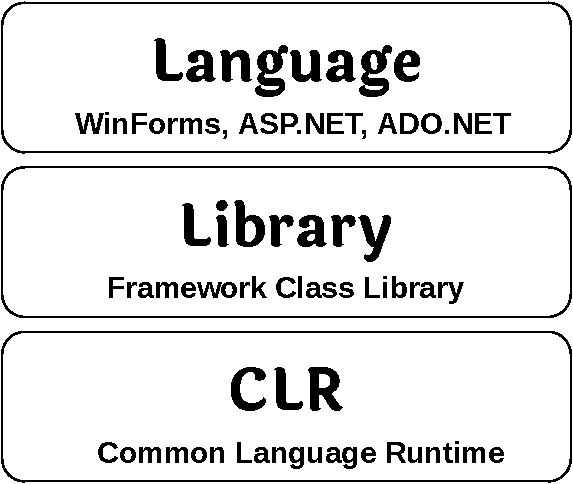
\includegraphics[width=0.7\textwidth]{dot-net-framework-architecture}
	\caption{.\ NET framework architecture}\label{fig:dot-net-architecture}
\end{figure}

The .\ Net Framework Architecture is the programming model for the .\ Net platform. It provides a managed execution environment, simplified development and deployment and integration with a wide variety of programming languages. The .\ Net Framework class library (FCL) is a comprehensive, object-oriented collection of reusable types that you can use to develop applications. The common language runtime (CLR) is the core runtime engine for executing applications in the .\ Net Framework. The CLR is fully protected from the outside environment and highly optimized within, taking advantage of the services that the CLR provides such as security, performance, deployment facilities, and memory management , including garbage collection.

%\subsubsection*{Components of .\ Net Framework}
%The .\ Net framework is composed of the following components:
%
%\begin{itemize}
%	\item \textit{ Common Language Runtime (CLR)}
%	\item \textit{Framework Class Library (FCL)} and
%	\item \textit{Languages (WinForms, ASP .\ NET, and ADO .\ NET, etc.\ )}.
%\end{itemize}
%
%
%\paragraph*{Common Language Runtime (CLR)}
%The Common Language Runtime (CLR) is an Execution Environment. It works as a layer between Operating Systems and the applications written in .\ Net languages that conforms to the Common Language Specification (CLS). The main function of CLR is to convert the Managed Code into native code and then execute the Program. The Managed Code compiled only when it needed, that is it converts the appropriate instructions when each function is called. CLR's Just In Time (JIT) compilation converts Intermediate Language (MSIL) to native code on demand at application run time.
%
%During the execution of the program, the CLR manages memory, Thread execution, Garbage Collection (GC), Exception Handling, Common Type System (CTS), code safety verifications, and other system services. The CLR defines the Common Type System (CTS), which is a standard type system used by all .\ Net languages. That means all .\ Net programming languages uses the same representation for common Data Types, so CLR is a language-independent runtime environment. The Common Language Runtime (CLR) environment is also referred to as a managed environment, because during the execution of a program it also controls the interaction with the Operating System.
%
%
%The CLR is an Execution Environment. Its main tasks are to convert the .\ Net Managed Code to native code, manage running code like a Virtual Machine and also controls the interaction with the Operating System.
%
%CLR manages Thread executions, Memory Management that is allocation of Objects and Buffers, Garbage Collection (GC) — Clean up the unused Objects and buffers, Exception Handling, CTS that is all .\ Net language that conforms to the Common Language Specification (CLS) have the same primitive Data Types, Code safety verification — code can be verified to ensure type safety, Language integration that is Common Language Runtime (CLR) follow a set of specification called Common Language Specification (CLS), this will ensure the interoperability between languages, Integrated security and other system services.
%
%\paragraph*{Framework Class Library (FCL)}
%The .\ Net Framework class library (FCL) provides the core functionality of .\ Net Framework architecture . The .\ Net Framework Class Library (FCL) includes a huge collection of reusable classes , interfaces, and value types that expedite and optimize the development process and provide access to system functionality.
%
%The .\ Net Framework class library (FCL) organized in a hierarchical tree structure and it is divided into Namespaces. Namespaces is a logical grouping of types for the purpose of identification. Framework class library (FCL) provides the consistent base types that are used across all .\ Net enabled languages. The Classes are accessed by namespaces, which reside within Assemblies. The System Namespace is the root for types in the .\ Net Framework. The .\ Net Framework class library (FCL) classes are managed classes that provide access to System Services . The .\ Net Framework class library (FCL) classes are object oriented and easy to use in program developments. Moreover, third-party components can integrate with the classes in the .\ Net Framework.
%
%


\subsubsection[CLR]{Common Language Runtime}
The ``Common Language Infrastructure'' or CLI is a platform in .\ Net architecture on which the .\ Net programs are executed.

The CLI has the following key features:

\begin{itemize}
	\item Exception Handling
	\item Garbage Collection
	\item Working with Various programming languages 
\end{itemize}

\subsubsection{Class Library}
The .NET Framework includes a set of standard class libraries. A class library is a collection of methods and functions that can be used for the core purpose.

For example, there is a class library with methods to handle all file-level operations. So, there is a method which can be used to read the text from a file. Similarly, there is a method to write text to a file.

Most of the methods are split into either the \texttt{System.*} or \texttt{Microsoft.* } namespaces\footnote{A namespace is a logical separation of methods.}. (The asterisk * just means a reference to all the methods that fall under the System or Microsoft namespace)



\subsubsection{Languages}
The types of applications that can be built in the .Net framework is classified broadly into the following categories

\begin{itemize}
	\item ADO.Net – This technology is used to develop applications to interact with Databases such as Oracle or Microsoft SQL Server: This is used for developing Forms-based applications, which would run on an end user machine. Notepad is an example of a client-based application.
	\item \texttt{ASP.Ne}t: This is used for developing web-based applications, which are made to run on any browser.
	\item \texttt{ADO.Net}: This technology is used to develop applications to interact with Databases such as Oracle or Microsoft SQL Server.
\end{itemize}



\subsection*{Common Language Specification (CLS)}
\begin{itemize}
	\item CLS is a set of basic language features that .\ Net Languages needed to develop Applications and Services, which are compatible with the .\ Net Framework.
	\item When there is a situation to communicate Objects written in different .\ Net Complaint languages, those objects must expose the features that are common to all the languages. 
	Common CLS ensures complete interoperability among applications, regardless of the language used to create the application.
	
\end{itemize}


\subsection*{Common Type System (CTS)}
CTS describes a set of types that can be used in different .\ Net languages in common. That is, the CTS ensure that objects written in different .\ Net languages can interact with each other. For Communicating between programs written in any .\ Net complaint language, the types have to be compatible on the basic level. 

These types can be Value Types or Reference Types. The Value Types are passed by values and stored in the stack. The Reference Types are passed by references and stored in the heap. CTS provides base set of Data Types which is responsible for cross language integration. The CLR can load and execute the source code written in any .\ Net language, only if the type is described in the CTS. Most of the members defined by types in the .\ Net FCL are CLS compliant Types.


\subsection*{Microsoft Intermediate Language (MSIL)}
\begin{itemize}
	\item MSIL stands for Microsoft Intermediate Language. 
	\item We can call it as Intermediate Language (IL) or Common Intermediate Language (CIL). 
	\item During the compile time, the compiler convert the source code into MSIL. 
	\item MSIL is a CPU-independent set of instructions that can be efficiently converted to the native code. 
	\item During the runtime the Common Language Runtime (CLR)'s Just In Time (JIT) compiler converts the MSIL code into native code to the Operating System.
\end{itemize}

When a compiler produces MSIL, it also produces Metadata. MSIL and Metadata are contained in a portable executable (PE) file. MSIL includes instructions for loading, storing, initializing, and calling methods on objects, as well as instructions for arithmetic and logical operations, control flow, direct memory access, exception handling, and other operations.

\subsection*{Just In Time Compiler (JIT)}
The .\ Net languages, which conforms to the Common Language Specification (CLS), uses its corresponding runtime to run the application on different Operating Systems. During the code execution time, the Managed Code compiled only when it is needed, that is it converts the appropriate instructions to the native code for execution just before when each function is called. This process is called Just In Time (JIT) compilation, also known as Dynamic Translation. With the help of Just In Time Compiler (JIT) the Common Language Runtime (CLR) doing these tasks.



The Common Language Runtime CLR provides various JIT compilers and each works on a different architecture depending on OS. That is why the same MSIL can be executed on different OS without rewriting the source code. JIT compilation preserves memory and save time during application initialization. 

\subsection*{Managed Code}
Managed Code in Microsoft .\ Net Framework, is the code that has executed by the Common Language Runtime (CLR) environment. On the other hand Unmanaged Code is directly executed by the computer's CPU. Data types, error-handling mechanisms, creation and destruction rules, and design guidelines vary between managed and unmanaged object models.

The benefits of Managed Code include programmers convenience and enhanced security. Managed code is designed to be more reliable and robust than unmanaged code, examples are Garbage Collection, Type Safety etc. The Managed Code running in a CLR cannot be accessed outside the runtime environment as well as cannot call directly from outside the runtime environment. This makes the programs more isolated and at the same time computers are more secure. Unmanaged Code can bypass the .\ Net Framework and make direct calls to the OS. Calling unmanaged code presents a major security risk.


\subsubsection*{Difference between managed and unmanaged code}
\paragraph*{What is Managed Code?}

Managed code is the code that is written to target the services of the managed runtime execution environment such as Common Language Runtime in .\ Net Technology.

\begin{figure}[ht!]
	\centering
	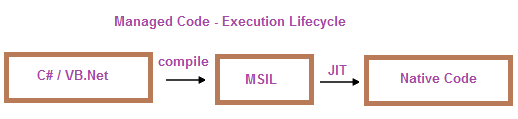
\includegraphics[width=0.7\linewidth]{managed-code}
	\caption[Managed Code]{Managed Code}
	\label{fig:managed-code}
\end{figure}

The Managed Code running under a CLR cannot be accessed outside the runtime environment as well as cannot call directly from outside the runtime environment. It refers to a contract of cooperation between natively executing code and the runtime. It offers services like garbage collection, run-time type checking, reference checking etc. By using managed code we can avoid many typical programming mistakes that lead to security holes and unstable applications, also, many unproductive programming tasks are automatically taken care of, such as type safety checking, memory management, destruction of unused objects etc.

\paragraph*{What is Unmanaged Code?}
Unmanaged code compiles straight to machine code and directly executed by the Operating System. The generated code runs natively on the host processor and the processor directly executes the code generated by the compiler. It is always compiled to target a specific architecture and will only run on the intended platform. If we want to run the same code on different architecture then we will have to recompile the code using that particular architecture.

Unmanaged executable files are basically a binary image, \texttt{x86} code, directly loaded into memory. This approach typically results in the fastest code execution, but diagnosing and recovery from errors might difficult and time-consuming in most cases. The memory allocation, type safety, security, etc needs to be taken care of by the programmer and this will lead unmanaged code prone to memory leaks like buffer overruns, pointer overrides etc.

All code compiled by traditional \texttt{C/C++} compilers are Unmanaged Code. COM components, ActiveX interfaces, and Win32 API functions are examples of unmanaged code. Managed code is code written in many high-level programming languages that are available for use with the Microsoft .\ Net Framework, including VB.\ Net, {\cs}, J{\texttt{\#}},  etc. Since Visual C++ can be compiled to either managed or unmanaged code it is possible to mix the two in the same application.


%\subsection*{.\ NET Components}
%The architecture of the .\ Net framework is based on the following key components:
%
%\subsubsection*{Common Language Runtime (CLR)}
%CLR handles execution of .\ NET code. The \textit{Common Language Infrastructure}
%or CLI is a platform on which the .\ Net programs are executed. It provides functionalities such as memory management, exception handling, debugging, security,
%thread execution, code execution, code safety, verification and compilation.
%
%The CLR also provides interoperability between different .\ Net languages. It
%provides a common environment for execution of different languages, such as {\cs},
%VB, VC++, etc.
%
%\subsubsection*{Class Library}
%The .\ Net Framework includes a set of standard class libraries. A class library is a collection of methods and functions that can be used for the core purpose.
%
%For example, there is a class library with methods to handle all file-level operations. So there is a method which can be used to read the text from a file. Similarly, there is a method to write text to a file.
%
%Most of the methods are split into either the \texttt{System.*} or \texttt{Microsoft.*} namespaces. (The asterisk \texttt{*} just means a reference to all the methods that fall under the System or Microsoft namespace)
%
%\subsubsection*{Languages}
%The types of applications that can be built in the .\ Net framework is classified broadly into the following categories.
%
%\paragraph*{WinForms}
%This is used for developing Forms-based applications, which would run on an end user machine. Notepad is an example of a client-based application.
%
%\paragraph*{ASP .\ NET}
%This is used for developing web-based applications, which are made to run on any browser such as Internet Explorer, Chrome or Firefox.
%	\begin{itemize}
%		\item The Web application would be processed on a server, which would have Internet Information Services Installed.
%		\item Internet Information Services or IIS is a Microsoft component which is used to execute an {Asp .\ Net} application.
%		\item The result of the execution is then sent to the client machines, and the output is shown in the browser.
%	\end{itemize}
%\paragraph*{ADO .\ NET}	
%This technology is used to develop applications to interact with Databases such as Oracle or Microsoft SQL Server.

%
%.\ NET Framework is designed to fulfill the following objectives:
%\begin{itemize}
%	\item To provide a consistent object-oriented programming environment whether object code is stored and executed locally, executed locally but web-distributed, or executed remotely.
%	
%	\item To provide a code-execution environment that minimizes software deployment and versioning conflicts.
%	
%	\item To provide a code-execution environment that promotes safe execution of code, including code created by an unknown or semi-trusted third party.
%	
%	\item To provide a code-execution environment that eliminates the performance problems of scripted or interpreted environments.
%	
%	\item To make the developer experience consistent across widely varying types of apps, such as Windows-based apps and Web-based apps.
%	
%	\item To build all communication on industry standards to ensure that code based on .\ Net Framework integrates with any other code.
%\end{itemize}
%
%
%
%\textbf{Features of .\ Net Framework}
%
%\begin{itemize}
%\item Less Coding and Increased Reuse of Code
%
%.\ Net framework supports Object-oriented programming (OOP) languages, which eliminates unnecessary codes and involves less coding. \.\ Net consists of reusable code and many reusable components. This translates into less time and consequently less cost to develop applications.
%
%\item Language-independent
%
%\.\ Net framework allows to develop Desktop, Web, Mobile and Console based applications. Also, it’s promoted as a language-independent framework, which means that development can happen in several compliant languages that include {\cs}, VB.\ Net, etc.
%
%\item Used for Service-Oriented Architecture
%
%.\ Net is often used for Web Services, WCF and Web API creation; which helps create REST API and SOAP based services that can communicate and transmit data utilizing standard Internet protocols.
%
%\item Easy Versioning \& Deployment Process
%
%With features like no-impact applications, private components, controlled code sharing, side-by-side versioning and partially trusted code, .\ Net framework makes deployment easier post development. The code execution environment supports safe code execution that minimizes software deployment and versioning conflicts. Moreover, it eliminates the performance problems of scripted or interpreted environments as well.
%
%\item Security
%
%.\ Net offers enhanced application security as web applications developed using ASP.\ Net have Windows confirmation and configuration. Managed code and CLR offer safeguard features like ‘role-based security’ and ‘code access security’.
%
%
%\item Multi-tiered Software Architecture
%
%.\ Net makes use of multi-tiered software architecture. It is known as multi-tiered because it physically separates functions for presentation, business logic and data management. It helps developers to build flexible applications. Moreover, developers also can add or edit a layer without being required to transform on the whole app.
%
%
%\item Feature-rich
%
%There are a variety of features which will be explored by the developers to make powerful apps. But then .\ Net Framework has been found to be a great platform for re-designing current applications in order to make it line up with the growing needs of an organization as well. For this, let us consider the case of its ‘rich toolbox’ and the ‘Designer’ in the visual studio. They let you access features such as automatic deployment, WYSIWYG editing, and drag-and-drop controls, etc. Any third-party control integration is also easily achievable with .\ Net Framework.
%
%\item Caching \& Exception Handling
%
%The caching \& exception handling features in .\ Net system, make your code more robust and easier-to-use.
%\end{itemize}

\subsection*{.\ Net Framework Design Principle}
The following design principles of the .\ Net framework is what makes it very relevant to create .\ Net based applications.

%\begin{description}
%	\item[Interoperability] The .\ Net framework provides a lot of backward support.
%	
%	\item [Portability].
%	
%	\item[Security]
%	
%	\item[Memory Management] The Common Language runtime does all the work or memory management. The .\ Net framework has all the capability to see those resources, which are not used by a running program. It would then release those resources accordingly. This is done via a program called the ``Garbage Collector" which runs as part of the .\ Net framework.
%	
%	The garbage collector runs at regular intervals and keeps on checking which system resources are not utilized, and frees them accordingly.
%	
%	\item[Simplified Deployment] The .\ Net framework also have tools, which can be used to package applications built on the .\ Net framework. These packages can then be distributed to client machines. The packages would then automatically install the application.
%\end{description}

The principal design features of Microsoft .\ Net Framework are:
\begin{multicols}{2}
\begin{itemize}
	\item \textit{Interoperability}
	\item \textit{Portability}
	\item \textit{Security}
	\item \textit{Language independence}
	\item \textit{Type safety}
	\item \textit{Memory management}
\end{itemize}
\end{multicols}


\subsubsection*{Interoperability}
Language interoperability is the ability of code to interact with code that is written using a different programming language. It can help maximize code reuse and, therefore, improve the efficiency of the development process. The .\ NET components can communicate with the existing COM components without migrating to those components into .\ NET. That means, this feature is a great help to reduce the migration cost and time. 

\subsubsection*{Portability}
 Applications built on the .\ Net framework can be made to work on any Windows platform. And now in recent times, Microsoft is also envisioning to make Microsoft products work on other platforms, such as iOS and Linux.
 
 \subsubsection*{Security}
  The .\ NET Framework has a good security mechanism. The inbuilt security mechanism helps in both validation and verification of applications. Every application can explicitly define their security mechanism. Each security mechanism is used to grant the user access to the code or to the running program.
  
  
 \subsubsection*{Language Independence}
 The .\ Net Framework is language independent. It is possible to use .\ Net from many programming languages because they have all agreed on some standards. This means that, as a programmer, we can develop in one of the many languages that target the .\ Net Framework, such as {\cs}, \texttt{C++/CLI}, Eiffel, F{\texttt{\#}, IronPython, IronRuby, PowerBuilder, Visual Basic, Visual COBOL, and Windows PowerShell. The .\ Net Framework presents a Common Type System (CTS) that characterizes every conceivable data sorts and programming builds bolstered by Common Language Runtime and how they might communicate with each other fitting in with CLI determination. Because of this feature, .\ Net Framework supports the exchange of types and object instances between libraries and applications written using any conforming .\ Net language.
 
 \subsubsection*{Type safety}
 Type-Safety is enforced by the CLR and the Language Compiler — in accordance to the CTS directives of the .\ Net Framework. Type-safe code cannot perform an operation on an object that is invalid for that object. This prevents ill-defined casts, wrong method invocations, and memory size issues when accessing an object. For example, if you have declared a variable as an integer, it cannot be assigned any value which is not an integer (by implicit conversion, or explicit conversion).
 
 \subsubsection*{Memory Management}
 The Common Language runtime does all the work or memory management. The .\ Net framework has all the capability to see those resources, which are not used by a running program. It would then release those resources accordingly. This is done via a program called the ``Garbage Collector", which runs as part of the .\ Net framework.
	
 The garbage collector runs at regular intervals and keeps on checking which system resources are not utilized, and frees them accordingly.
 

\section{Introduction to {\cs} and VB}
\subsection{{\cs}}
 {{\cs}} is a modern, general-purpose, object-oriented programming language developed by Microsoft and approved by European Computer Manufacturers Association (ECMA) and International Standards Organization (ISO).

{\cs} was developed by \textit{Anders Hejlsberg} and his team during the development of .\ Net Framework. It is based on C++ and Java, but it has many additional extensions used to perform component oriented programming approach.

{\cs} is designed for Common Language Infrastructure (CLI), which consists of the executable code and runtime environment that allows use of various high-level languages on different computer platforms and architectures.

\subsubsection*{{\cs} Features}
\begin{itemize}
	\item \textit{Simple}
	
	{\cs} is a simple language in the sense that it provides structured approach (to break the problem into parts), rich set of library functions, data types etc.
	
	\item \textit{Modern Programming Language}

	{\cs} programming is based upon the current trend and it is very powerful and simple for building scalable, interoperable and robust applications.
	\item \textit{Object-Oriented}
	
		{\cs} is object-oriented programming language. OOPs makes development and maintenance easier where as in Procedure-oriented programming language it is not easy to manage if code grows as project size grow.
		
	\item \textit{Type Safe}
	
	{\cs} type safe code can only access the memory location that it has permission to execute. Therefore it improves a security of the program.
	\item \textit{Interoperability}
	
	Interoperability process enables the {\cs} programs to do almost anything that a native C++ application can do.
	\item  Scalable and Updateable
	
	{\cs} is automatic scalable and updateable programming language. For updating our application we delete the old files and update them with new ones.
		
	\item \textit{Structured Programming Language}
	
	{\cs} is a structured programming language in the sense that we can break the program into parts using functions. So, it is easy to understand and modify.
	
	\item \textit{Rich Library}
	
	{\cs} provides a lot of inbuilt functions that makes the development fast.
	
\end{itemize}

%https://www.vbtutor.\ /lesson1.html
%Lesson 1 : Introduction to Visual Basic
%https://www.vbtutor.\ /lesson1.html
%2008 Dr.Liew Voon Kiong. 
\subsection{VB (Visual Basic) .\ NET}

Visual Basic is a third-generation event-driven programming language first released by Microsoft in 1991. It evolved from the earlier {DOS} version called {BASIC}. BASIC means \textit{Beginners' All-purpose Symbolic Instruction Code}. % Since then Microsoft has released many versions of Visual Basic, from Visual Basic 1.0 to the final version Visual Basic 6.0. Visual Basic is a user-friendly programming language designed for beginners, and it enables anyone to develop GUI window applications easily. 

VB .\ NET is a fully object-oriented programming language implemented in the .\ NET Framework. It was created to cater for the development of the web as well as mobile applications.

VB .\ Net is an update to Visual Basic that targets Microsoft .\ Net Framework. VB .\ Net has a lot of similarities to Visual Basic but also some differences. VB .\ Net is an object-oriented language, which supports the abstraction, encapsulation, inheritance, and polymorphism features. It is the most productive tool for rapidly creating a wide range of Windows, Web, Mobile, and Office applications built on the .\ Net Framework.

The Visual Basic language is designed to be human-readable and accessible to everyone from novice programmers to advanced system architects. All of this is built on top of the .\ Net Framework, which guarantees that programs written in Visual Basic run with unsurpassed scalability and reliability. The .\ Net Framework provides VB .\ Net programmers with the ability to create fully object oriented programs (OOPs), just like the ones created using Java, {\cs} or C\texttt{++}. Also programs written in VB.\ Net will interoperate seamlessly with programs written in any other .\ Net languages such as Visual {\cs}, Visual J\texttt{\#}, or Visual C\texttt{++}.

\subsubsection*{Featues of VB .\ Net}
VB .\ NET comes loaded with numerous features that have made it a popular programming language amongst programmers worldwide. These features include the following
\begin{multicols}{2}
\begin{itemize}
	\item VB.NET is not case-sensitive 
	\item It is an object-oriented programming language
	\item Garbage collection
	\item Events management
	\item Windows Forms
	\item Support for web application development
\end{itemize}
\end{multicols}


\section{Feature of Object Oriented Programming}

\subsection*{Object}	
Object is a collection of number of entities. Objects take up space in the memory. Objects are instances of classes. When a program is executed, the objects interact by sending messages to one another. Each object contain data and code to manipulate the data. Objects can interact without having know details of each others data or code.

\subsection*{Class}
Class is a collection of objects of similar type. Objects are variables of the type class. Once a class has been defined, we can create any number of objects belonging to that class. Classes are user define data types.
	 
\subsection*{Data Abstraction and Encapsulation}
 Combining data and functions into a single unit called class and the process is known as Encapsulation. Data encapsulation is important feature of a class. Class contains both data and functions. Data is not accessible from the outside world and only those function which are present in the class can access the data. The insulation of the data from direct access by the program is called data hiding or information hiding. Hiding the complexity of program is called Abstraction and only essential features are represented. In short, we can say that internal working is hidden.
	 
\subsection*{Dynamic Binding}
Refers to linking of function call with function definition is called binding and when it is take place at run time called dynamic binding.
	 
\subsection*{Message Passing} 
The process by which one object can interact with other object is called message passing.
	
\subsection*{Inheritance}
It is the process by which object of a class acquire the properties or features of objects of another class. The concept of inheritance provide the idea of re-usability means we can add additional features to an existing class without modifying it. This is possible by deriving a new class from the existing one. The new class will have the combined features of both the classes.

\subsection*{Polymorphism}
An operation may exhibit different behaviors in different instances. The behavior depends upon the types of data used in the operation. Its types:
 \begin{itemize}
 	\item Static / Compile Time Polymorphism.
 	\begin{itemize}
 		\item Method Overloading and 
 		\item Operator Overloading
 	\end{itemize}
 	\item Dynamic / Runtime Polymorphism.
 	
 \end{itemize}
 
\section{Scope of .\ Net  Technology}
Following are the scope of .\ Net Technology:
\begin{multicols}{2}
\begin{itemize}
		\item Cross platform mobile application development
		\item Desktop application
		\item Web application
		\item Web services
		\item Websites
		\item Games 
		\item Virtual Reality (VR) application
		\item Database application, etc.
\end{itemize}
\end{multicols}



 % ch-1: Overview of VB .\ NET and C\# .\ NET Language
\chapter{ Language Basics}
\section{Variables and Data Types}
\subsection{Variables}
%https://www.javatpoint.com/csharp-variables
%{\cs} Variable

A variable is a name of memory location. It is used to store data. Its value can be changed and it can be reused many times. It is a way to represent memory location through symbol so that it can be easily identified. The basic variable type available in {\cs} can be categorized as:


	\begin{table}[hb]
		\centering
		\begin{tabular}{ll}
			\toprule
			\textbf{Variable Type} & \textbf{Example}                 \\ \midrule
			Decimal types          & decimal                          \\
			Boolean types          & True or false value, as assigned \\
			Integral types         & int, char, byte, short, long     \\
			Floating point types   & float and double                 \\
			Nullable types         & Nullable data types              \\ \bottomrule
		\end{tabular}
	\end{table}

%https://www.tutorialspoint.com/csharp/csharp_variables.htm
%{\cs} - Variables
{\cs} also allows defining other value types of variable such as \verb|enum| and reference types of variables such as \verb|class|.

\subsubsection*{Variable Declaration in {\cs}}
Syntax for variable definition in {\cs} is:
\begin{lstlisting}[numbers=none]
	<data_type> <variable_list>;
\end{lstlisting}

Here, \verb|data_type| must be a valid {\cs} data type including char, int, float, double, or any user-defined data type, and \verb|variable_list| may consist of one or more identifier names separated by commas.

Some valid variable definitions are shown here:
\begin{lstlisting}[numbers=none]
int i, j, k;
char c, ch;
float f, salary;
double d;
\end{lstlisting}

\subsubsection*{Variable Declaration in VB .\ NET}
The \texttt{Dim} statement is used for variable declaration and storage allocation for one or more variables. The Dim statement
is used at \textit{module}, \textit{class}, \textit{structure}, \textit{procedure} or \textit{block level}.
Syntax for variable declaration in VB .\ Net is:
\begin{lstlisting}[style=vb, numbers=none]
	DIM <variable_name> As <data_type>
\end{lstlisting}

Some valid variable declarations along with their definition are shown here:
\begin{lstlisting}[style=vb, numbers=none]
' VB
Dim StudentID As Integer
Dim StudentName As String
Dim Salary As Double
Dim count1, count2 As Integer
Dim status As Boolean
Dim exitButton As New System.Windows.Forms.Button
Dim lastTime, nextTime As Date
\end{lstlisting}

\subsubsection*{Variable Initialization}
Variables are initialized (assigned a value) with an equal sign followed by a constant expression. The general form of initialization is:

\begin{lstlisting}[numbers=none]
variable_name = value;
\end{lstlisting}

Variables can be initialized in their declaration. The initializer consists of an equal sign followed by a constant expression as:

\begin{lstlisting}[style=vb, numbers=none]
' C#
<data_type> <variable_name> = value;

' VB
DIM <variable_name> As <data_type> = value
\end{lstlisting}

Variable can be initialized at the time of declaration as follows:
\begin{lstlisting}[numbers=none]
// C#
string studentName = "Jeevan";
\end{lstlisting}

\begin{lstlisting}[style=vb, numbers=none]
' VB
Dim semesterID As Integer = 8
Dim teacherName As String = "Madan Uprety"
\end{lstlisting}
\subsubsection*{Rules for defining variables}
\begin{itemize}
	\item A variable can have alphabets, digits and underscore.

	\item A variable name can start with alphabet and underscore only. It can't start with a digit.

	\item No white space is allowed within variable name.

	\item A variable name must not be any reserved word or keyword e.g. char, float etc.
\end{itemize}

Some examples are:
\begin{lstlisting}[numbers=none]
// C#
int semesterId = 8, rollNo = 69;
byte x = 22;
double pi = 3.14159;
char name = `x';
\end{lstlisting}

\subsection{Data Types}
%Mithun Kumar & jit_t
%https://www.geeksforgeeks.org/c-sharp-data-types/
%{\cs} | Data Types
%GeeksforGeeks

Data types specify the type of data that a valid {\cs} variable can hold. {\cs} is a strongly typed programming language because in {\cs}, each type of data (such as integer, character, float, and so forth) is predefined as part of the programming language and all constants or variables defined for a given program must be described.

\subsubsection*{Value Data Types}

%	https://www.geeksforgeeks.org/c-sharp-data-types/
%	Mithun Kumar & jit_t
%	{\cs} | Data Types
	In {\cs}, the Value Data Types will directly store the variable value in memory and it will also accept both signed and unsigned literals. The derived class for these data types are \verb|System.ValueType|


	\subsubsection*{ Reference Data Type}

	The reference types do not contain the actual data stored in a variable, but they contain a reference to the variables.

	In other words, they refer to a memory location. Using multiple variables, the reference types can refer to a memory location. If the data in the memory location is changed by one of the variables, the other variable automatically reflects this change in value. Example of built-in reference types are: object, dynamic, and string.

		\paragraph*{Object Type}

		In {\cs}, all types, predefined and user-defined, reference types and value types, inherit directly or indirectly from Object. So basically it is the base class for all the data types. Before assigning values, it needs type conversion. When a variable of a value type is converted to object, it’s called boxing. When a variable of type object is converted to a value type, it’s called unboxing. Its type name is \verb|System.Object|.


\paragraph*{String Type}
It represents a sequence of Unicode characters and its type name is \texttt{System.String}. So, \texttt{string} and \texttt{String} are equivalent. Example:
		\begin{lstlisting}
// creating through string keyword
	string s1 = "Corona";

// creating through String class
	String s2 = "COVID-19";
\end{lstlisting}

 \paragraph*{Dynamic Type}
	You can store any type of value in the dynamic data type variable. Type checking for these types of variables takes place at run-time.

\begin{lstlisting}
// Syntax
	dynamic <variable_name> = value;

// Example
	dynamic d = 69;
\end{lstlisting}

Dynamic types are similar to object types except that type checking for object type variables takes place at compile time, whereas that for the dynamic type variables takes place at run time.


\subsubsection*{Pointer Type}
%	https://www.tutorialspoint.com/csharp/csharp_data_types.htm
%	{\cs} - Data Types

	Pointer type variables store the memory address of another type. To get the pointer details we have a two symbols: ampersand (\&) and asterisk (*).

\begin{itemize}
		\item 	ampersand (\&): It is Known as Address Operator. It is used to determine the address of a variable.

		\item 	asterisk (*): It also known as Indirection Operator. It is used to access the value of an address.

\begin{lstlisting}[numbers=none]
// Syntax
	type* identifier;

// Example
	int* p1, p;   // Valid syntax
	int *p1, *p;   // Invalid
\end{lstlisting}


\end{itemize}




\section{String and String Builder}
%Mithun Kumar
%GeeksforGeeks
%{\cs} | String
%https://www.geeksforgeeks.org/c-sharp-string/
%accessed 27 april 2020
\subsection{String}
 String is a sequence of Unicode characters or array of characters. The array of characters is also termed as the text. So the string is the representation of the text.

 A string is represented by class \verb|System.String|. The \verb|string| keyword is an alias for \verb|System.String| class and instead of writing \verb|System.String| one can use \verb|String| which is a shorthand for \verb|System.String| class. So, we can say \verb|string| and \verb|String| both can be used as an alias of \verb|System.String |class. So \verb|string| is an object of \verb|System.String |class.

 \begin{lstlisting}[numbers=none]
 // Example:

 // creating the string using string keyword
 string courseName = "BCA";

 // creating the string using String class
 String semester = "Semester-VIII";

 // creating the string using String class
 System.String calenderYearNP ="2077 B.S.";
 \end{lstlisting}

The String class is defined in the \verb|.NET| base class library. In other words a String object is a sequential collection of \verb|System.Char| objects which represents a string. The maximum size of String object in memory is 2GB or about 1 billion characters. \verb|System.String| class is \textbf{immutable}, i.e once created its state cannot be altered.

\subsubsection*{String Class Properties}
The String class has two properties as follows:
\begin{itemize}
	\item Chars: It is used to get the Char object at a specified position in the current String object.
	\item Length: It is used to get the number of characters in the current String object.
\end{itemize}

\subsection{String Builder}

A string instance is immutable. Immutable means once we create a string object we cannot modify the value of the string Object in the memory. Any operation that appears to modify the string, it will discard the old value and it will create new instance in memory to hold the new value.

The \texttt{System.Text.StringBuilder} is mutable, that means once we create \texttt{StringBuilder} object we can perform any operation that appears to change the value without creating new instance for every time. It can be modified in any way and it doesn't require creation of new instance.

\begin{lstlisting}
// String Example

string colors;
colors += "red";
colors += "blue";
colors += "green";
\end{lstlisting}

In the above code, string color will alter 3 times, each time the code perform a string operation \verb|(+=)|. That mean 3 new string created in the memory. When you perform repeated operation to a string, the overhead associated with creating a new String object can be costly.

\begin{lstlisting}
// StringBuilder Example

StringBuilder sb = new StringBuilder("");
sb.Append("red");
sb.Append("blue");
sb.Append("green ");
string colors = sb.ToString();
\end{lstlisting}

In the above code the \texttt{StringBuilder} object will alter 3 times, each time the code attempt a \texttt{StringBuilder} operation without creating a new object. That means, using the \texttt{StringBuilder} class can boost performance when concatenating many strings together in a loop.

But immutable objects have some advantages also, such as they can be used across threads without fearing synchronization problems. On the other hand, when initializing a \texttt{StringBuilder}, you are going down in performance. Also many actions that you do with string can't be done with \texttt{StringBuilder} object.

	\begin{table}[ht]
	\centering
	\caption{Differences between String and StringBuilder class}\label{tab:string-vs-string-builder}
	\begin{tabular}{p{5.5cm}p{5.5cm}}
	\toprule % <-- Toprule here
		\textbf{String} & \textbf{StringBuilder} \\
		\midrule % <-- Midrule here
		\texttt{System.String} is immutable  &
		\texttt{System.StringBuilder} is mutable \\
	
Concatenation is used to combine two strings & Append method is used\\

 The first string is combined to the other string by creating a new copy in the memory as a string object, and then the old string is deleted
  & Insertion is done on the existing string. \\

  \texttt{String} is efficient for small string manipulation & \texttt{StringBuilder} is more efficient in case large amounts of string manipulations have to be performed \\
	  \bottomrule %% <-- Bottomrule here
	\end{tabular}
	\end{table}


\section{Boxing and Unboxing}

{\cs} Type System contains three Types, they are:
\begin{itemize}
	\item Value Types,
	\item Reference Types and
	\item Pointer Types.
\end{itemize}
{\cs} allows us to convert a Value Type to a Reference Type, and back again to Value Types. The operation of Converting a Value Type to a Reference Type is called \textbf{Boxing} and the reverse operation is called \textbf{Unboxing}.

\subsection{Boxing}
\begin{lstlisting}
int Val = 1;
Object Obj = Val; //Boxing
\end{lstlisting}

The first line we created a Value Type \texttt{Val} and assigned a value to Val. The second line, we created an instance of \texttt{Object Obj} and assign the value of Val to Obj. From the above operation \verb|Object Obj = i| we saw converting a value of a Value Type into a value of a corresponding Reference Type. These types of operation is called Boxing.

\subsection{UnBoxing}
\begin{lstlisting}
int Val = 1;
Object Obj = Val; //Boxing
int i = (int)Obj; //Unboxing
\end{lstlisting}

The first two line shows how to Box a Value Type. The next line int \texttt{i = (int) Obj} shows extracts the Value Type from the Object. That is converting a value of a Reference Type into a value of a Value Type. This operation is called UnBoxing.

Boxing and UnBoxing are computationally expensive processes. When a value type is boxed, an entirely new object must be allocated and constructed, also the cast required for UnBoxing is also expensive computationally.

	\begin{table}[h]
	\centering
	\caption{Difference between boxing and unboxing.}\label{tab:boxing-vs-unboxing}
	\begin{tabular}{p{5.5cm}p{5.5cm}}
  \toprule
		\textbf{Boxing} & \textbf{Unboxing} \\
		\midrule
		It convert value type into an object type.  & It convert an object type into value type. \\
		Boxing is an implicit conversion process. & Unboxing is the explicit conversion process.\\
		Here, the value stored on the stack copied to the object stored on the heap memory. & Here, the object stored on the heap memory copied to the value stored on the stack . \\
	\bottomrule
	\end{tabular}
\end{table}

\section{Operators}
An operator is a symbol that tells the compiler to perform specific mathematical or logical manipulations. {\cs} has rich set of built-in operators and provides the following type of operators.


\subsection{Arithmetic Operators}
The arithmetic operators perform arithmetic operations on all the numeric type operands such as sbyte, byte, short, ushort, int, uint, long, ulong, float, double, and decimal.

\begin{table}[htb!]
	\centering
	\begin{tabular}{p{0.8cm} p{6cm}p{3cm}}
		\toprule
		Operator     & Description                                                 & Example                    \\ \midrule
		\texttt{+}   & Adds two operands                                           & \texttt{int x = 30 + 6;}   \\
		\texttt{-}   & Subtracts second operand from the first                     & \texttt{int x = 70 - 1; }  \\
		\texttt{*}   & Multiplies both operands                                    & \texttt{int x = 4 * 9;}    \\
		\texttt{/}   & Divides numerator by denominator                            & \texttt{int x = 138 / 2;}  \\
		\texttt{\%}  & Modulus Operator and remainder of after an integer division & \texttt{int x = 69 \% 36;} \\
		\texttt{++}  & Increment operator increases integer value by one           & \texttt{x++;}              \\
		\texttt{x--} & Decrement operator decreases integer value by one           & \texttt{x--;}              \\ \bottomrule
	\end{tabular}
\end{table}

\subsection{Relational Operators}
Relational operators are used to check the relationship between two operands. If the relationship is true the result will be \verb|true|, otherwise it will result in \verb|false|. Relational operators are used in decision-making and loops. Table {\ref{tab:comparison-operator}} shows list of comparison operators.

\begin{table}[ht!]
	\centering
	\caption{Comparison Operators.}\label{tab:comparison-operator}
	\begin{tabular}{p{1cm}p{3.5cm}p{5cm}}
		\toprule
		\textbf{Operator}     & \textbf{Name}                     & \textbf{Example}  \\ \midrule
		\texttt{==}  & Equal to                 & \texttt{6 == 4} evaluates to false  \\
		\texttt{>}   & Greater than             & \texttt{3 > -1} evaluates to true   \\
		\texttt{< }  & Less than                & \texttt{5 < 3} evaluates to false   \\
		\texttt{>=}  & Greater than or equal to & \texttt{4 >= 4} evaluates to true   \\
		\texttt{<= } & Less than or equal to    & \texttt{5 <= 3} evaluates to false  \\
		\texttt{!=}  & Not equal to             & \texttt{10 != 2} evaluates to true  \\ \bottomrule
	\end{tabular}
\end{table}

\subsection{Logical Operators}
Logical operators are used to perform logical operation such as and, or. Logical operators operates on boolean expressions (true and false) and returns boolean values. Logical operators are used in decision-making and loops. Table {\ref{tab:logical-operator}} shows list of logical operators.

\begin{table}[hb]
	\centering
	\caption{Logical Operators.}\label{tab:logical-operator}
\begin{tabular}{p{1cm}p{6cm}p{3cm}}
	\toprule
	Operator      & Description                                                                                                  & Example            \\ \midrule
	\texttt{\&\&} & Computes the logical AND of its bool operands. Returns true both operands are true, otherwise returns false. & \texttt{x \&\& y}; \\
	\texttt{||}     & Computes the logical OR of its bool operands. Returns true when any one operand is true.                     & \texttt{x || y};    \\ \bottomrule
\end{tabular}
\end{table}

\subsection{Compound Assignment Operators}
	 The assignment operator \texttt{=} assigns its right-hand value to its left-hand variable, property, or indexer. It can also be used with other arithmetic, Boolean logical, and bitwise operators. Table {\ref{tab:compound-assignment-operator}} shows list of compound assignment operators.
	 \begin{table}[ht]
	 	\centering
	 	\caption{Compound Assignment Operators.}\label{tab:compound-assignment-operator}
	 \begin{tabular}{p{4cm}p{3cm}p{3cm}}
	 	\toprule
	 	Operator & Example  & Same As    \\ \midrule
	 	=        & x = 6    & x = 6      \\
	 	+=       & x += 4   & x = x + 4  \\
	 	-=       & x -= 6   & x = x - 6  \\
	 	*=       & x *= 9   & x = x * 9  \\
	 	/=       & x /= 7   & x = x / 7  \\
	 	\%=      & x \% = 2 & x = x \% 2 \\ \bottomrule
	 \end{tabular}
	 \end{table}


\subsection{Ternary Operator}
The ternary operator \verb|? :| operates on three operands. It is a shorthand for if-then-else statement.

\begin{lstlisting}[numbers=none]
// Syntax: ternary operator
variable = Condition? Expression1 : Expression2;
\end{lstlisting}

The ternary operator works as follows:
\begin{itemize}
	\item If the expression stated by Condition is \verb|true|, the result of \verb|Expression1| is assigned to variable
	\item If it is \verb|false|, the result of \verb|Expression2| is assigned to variable
\end{itemize}

\begin{lstlisting}[numbers=none]
// Example
int number = 18;
string result;

result = (number % 2 == 0)? "Even Number" : "Odd Number";
\end{lstlisting}

\section{Control statements}
Program needs a way to make decisions as it makes progress through the execution of code. This is where control flow comes into play. The program control flow is provided to us by the use of control statements. These are the special keywords in the {\cs} language that allow the programmer to set up things like branching, looping, and even entire jumps to new points in the program during execution.
Control statements:
\begin{itemize}
	\item \textbf{Selection Statements}: This consists of \verb|if|, \verb|else|, \verb|switch|, and \verb|case| branching

	\item \textbf{Iteration Statements}: This consists of \verb|do|, \verb|for|, \verb|foreach|, and \verb|while| looping

	\item \textbf{Jump Statements}: This consists of \verb|break|, \verb|continue|, \verb|return|, and \verb|goto| statements
\end{itemize}

\subsection{Conditional Statements}
A conditional statement decides whether to execute code based on conditions. The if statement and the switch statement are the two types of conditional statements in {\cs}.

\subsection{{\cs}}
\subsubsection*{if statement}
The if statement selects a branch for execution based on the value of a Boolean expression.
\begin{lstlisting}[numbers=none]
// C#
// Syntax: if statement
if (condition) {
// Statement(s)
} else {
// Statement(s)
}
\end{lstlisting}

The if statement evaluates its condition expression to determine whether to execute the if-body. Optionally, an else clause can immediately follow the if body, providing code to execute when the condition is false. Making the else-body another if statement creates the common cascade of \verb|if, else if, else if, else if, else| statements.

\subsubsection*{switch statement}
Switch statement can be used to branch the execution of a program to a set of statements that are inside of a case label, which is created with the keyword \verb|case|. The {\cs} switch statement does this by matching the value inside the switch against the values that you specify in each case label.

\begin{itemize}
	\item Restricted to integers, characters, strings, and enums
	\item Case labels are constants
	\item Default label is optional
\end{itemize}

\begin{lstlisting}[numbers=none]
// Syntax: switch statement
switch (expression) {
case value1:
// statements
	break;

case value2:
// statements
	break;
.
.
case valueN:
// statements
	break;
default:
// default statement
}
\end{lstlisting}

\subsection{VB}

\subsubsection*{If ... Then Statement}
\begin{lstlisting}[style=vb, numbers=none]
' VB Syntax: if ... then statement
If (condition) Then
	' Statement(s)
End IF
\end{lstlisting}

\subsubsection{If ... Then ... Else Statement}
An If statement can be followed by an optional Else statement, it executes when the Boolean expression is false.
\begin{lstlisting}[style=vb, numbers = none]
If (boolean_expression) Then
	'execute if Boolean expression is true
Else
	'execute if Boolean expression is false
End If
\end{lstlisting}

\subsubsection{If ...  ElseIf ... Else Statement}
An If statement can be followed by an optional Else if...Else statement, which is very useful to test various conditions using single If...Else If statement.
\begin{lstlisting}[style=vb, numbers=none]
' Syntax for if... else if ... else
If(boolean_expression 1)Then
	' Executes when the boolean expression 1 is true
ElseIf( boolean_expression 2)Then
	' Executes when the boolean expression 2 is true
ElseIf( boolean_expression 3)Then
	' Executes when the boolean expression 3 is true
Else
	' Executes when the none of the above condition is true
End If
\end{lstlisting}

\subsubsection{Nested If Statement}
It is always legal in VB.Net to nest If-Then-Else statements, which means you can use one If or ElseIf statement inside another If ElseIf statement(s).

\begin{lstlisting}[style=vb, numbers=none]
If(boolean_expression 1)Then
 	'Executes when the boolean expression 1 is true
		If(boolean_expression 2)Then
			'Executes when the boolean expression 2 is true
		End If
End If
\end{lstlisting}


\subsubsection{Select Case Statement}
A Select Case statement allows a variable to be tested for equality against a list of values. Each value is called a case, and the variable being switched on is checked for each select case.
\begin{lstlisting}[style=vb, numbers=none]
' VB: Syntax: Select Case
Select (expression)
	Case case1
		'statements
	Case caseN
		'statements
	Case Else
		'statements
End Select
\end{lstlisting}

\subsection*{Loops in VB}
\subsubsection*{Do loop}
It repeats the enclosed block of statements while a Boolean condition is True or until the condition becomes True. It could be terminated at any time with the Exit Do statement.

\begin{lstlisting}[style=vb, numbers = none]
' Syntax: sDo loop	
Do (While | Until) (condition)
	' statements
	' Continue Do
	' statements 
	' Exit Do 
	' statements
	Loop
	' -or-
Do
	 'statements
	' Continue Do
	' statements 
	' Exit Do 
	' statements
	Loop (While | Until ) (condition)
\end{lstlisting}


\subsection{Iteration statements}
An iteration statement creates a loop of code to execute a variable number of times. Iterating is also known as looping. Looping is when you need or want to execute a piece of code many times. The \verb|for| loop, the \verb|do| loop, the \verb|while| loop, and the \verb|foreach| loop are the iteration statements in {\cs}.

\subsubsection{do ... while loop}
The \verb|do...while| loop always runs its body once. After its first run, it evaluates its condition to determine whether to run its body again. If the \verb|condition| is true, the body executes. If the condition evaluates to true again after the body has run, the body executes again. When the condition evaluates to false, the \verb|do...while| loop ends.
\begin{lstlisting}[numbers=none]
// Syntax: do ... while loop
do {
	statement;
} while (condition);
\end{lstlisting}

\subsubsection{for loop}
For loop repeats the execution of a statement until a specified \verb|condition| is false. It proves most useful when the developer knows the exact number of necessary iterations. Its statements initialize the iteration variable, state the related condition, and state the iteration operation. Note that all statements within a for statement are optional, and omissions can create infinite loops.

\begin{lstlisting}[numbers=none]
// Syntax: for loop
for (initialization; condition; iterator) {
	statement;
}
\end{lstlisting}

\subsubsection{foreach loop}
The \verb|foreach| statement is similar to the for statement in that both allow code to iterate over the items of collections, but the foreach statement lacks an iteration index, so it works even with collections that lack indices altogether. When the collection is fully traversed, the loop will terminate.
\begin{lstlisting}[numbers=none]
// Syntax: foreach loop
foreach(int element in collection) {
	statement;
}
\end{lstlisting}


\subsubsection{while}
The while loop executes a statement(s) while a condition evaluates to true.
\begin{lstlisting}[numbers=none]
// Syntax: while loop
while (statement) {
statement;
}
\end{lstlisting}

\subsection{Jump statements}
 Jump statements are used to transfer control from one point to another point in the program. There are five keywords in the Jump Statements: \texttt{break, continue, goto, return and throw}


\subsubsection*{break statement}
The break statement is used to terminate the loop or statement in which it present. After that, the control will pass to the statements that present after the break statement, if available. If the break statement present in the nested loop, then it terminates only those loops which contains break statement.

\subsubsection*{continue statement}
This statement is used to skip over the execution part of the loop on a certain condition. After that, it transfers the control to the beginning of the loop. Basically, it skips its following statements and continues with the next iteration of the loop.

\subsubsection*{goto statement}
This statement is used to transfer control to the labeled statement in the program. The label is the valid identifier and placed just before the statement from where the control is transferred.

\subsubsection*{return statement}
This statement terminates the execution of the method and returns the control to the calling method. It returns an optional value. If the type of method is void, then the return statement can be excluded.

\subsubsection*{throw statement}
This is used to create an object of any valid exception class with the help of \verb|new| keyword manually. The valid exception must be derived from the Exception class.


\section{Arrays and Strings}

Arrays represent a set of items all belonging to the same type. The declaration itself may use a variable or a constant to define the length of the array. However, an array has a set length and it cannot be changed after declaration.

\subsection{Array Declaration}
The syntax for declaring an array follows:

\begin{lstlisting}[numbers=none]
// Syntax
datatype[] arrayName;
\end{lstlisting}
Where,
\begin{itemize}
	\item \texttt{datatype}: defines the element type of the array
	\item \texttt{[]}: defines the size of the array
	\item \texttt{arrayName}: is the Name of array
\end{itemize}

\begin{lstlisting}[numbers=none]
// Example
int[] totalCount; // can store int values
string[] affectedCountries; // can store string values
double[] economicLoss; // can store double values
CoronaVirus[] covid19; // can store instances of CoronaVirus class which is a custom class
\end{lstlisting}
\emph{Only Declaration of an array doesn’t allocate memory to the array. For that array must be initialized.}

\subsection{Array Initialization}
An array is a reference type so the \verb|new| keyword used to create an instance of the array. We can assign initialize individual array elements, with the help of the index.

\begin{lstlisting}[numbers=none]
// Syntax:
datatype[] arrayName= new datatype[size];
\end{lstlisting}
Where,
\begin{itemize}
	\item \texttt{datatype}: specifies the type of data being allocated
	\item \texttt{size}: specifies the number of elements in the array
	\item \texttt{arrayName}: is the name of array variable
	\item \texttt{new}: allocates memory to an array according to its size
\end{itemize}


\begin{lstlisting}[numbers=none]
 // different ways of array declaration and initialization

// define array without assigning value
int[] year = new int[4];

// define array and assign value at the same time
int[] year = new int[4] {2074, 2075, 2076, 2077};

// defining array with elements
// that indicates the size of an array
int[] year = {2074, 2075, 2076, 2077};
\end{lstlisting}


\noindent Arrays are categorized as one-dimensional, multi-dimensional, or jagged. In the creation of an array, its number of dimensions and their length are set.

\subsubsection*{One Dimensional Array}
This array contains only one row for storing the values. All values of this array are stored contiguously starting from 0 to the array size.
\begin{lstlisting}[numbers=none]
//Syntax: 1-D array declaration
double[] xx = new double[69];
\end{lstlisting}


\subsubsection*{Multidimensional Arrays}
The multi-dimensional array contains more than one row to store the values. It is also known as a \textbf{Rectangular Array} in {\cs} because it’s each row length is same. It can be a 2D-array or 3D-array or more. Nested loop is required inorder to access multidimensional array.
\begin{lstlisting}[numbers=none]
// creates a two-dimensional array of
// four rows and three columns.
int[, ] arrayName = new int[4, 3];

//creates an array of three dimensions, 5, 3, and 2
int[, , ] arrayName = new int[5, 3, 2];

 // one comma indicates 2-dimensional
 // and two commas indicate 3-dimensional.
\end{lstlisting}


\subsubsection*{Jagged Arrays}
A jagged array is an array whose elements are themselves arrays, not all necessarily of the same length. This is declared in the format

\begin{lstlisting}[numbers=none]
//jagged array declaration
datatype[][] arrayName
\end{lstlisting}
\noindent where, we have \verb|[][]| instead of \verb|[,]|.\\

\noindent Example,

\begin{lstlisting}[numbers=none]
// Example
int[][] Jag = new int[3][];
\end{lstlisting}

 \noindent \break Before you can use Jag, its elements must be initialized. You can initialize the elements like this:
\begin{lstlisting}[numbers=none]
Jag[0] = new int[5]; // array of 5 integers
Jag[1] = new int[4]; // array of 4 integers
Jag[2] = new int[2]; // array of 2 integers
\end{lstlisting}

\noindent \break Each of the elements is a single-dimensional array of integers.\\

\noindent We can initialize the array when we create it:
\begin{lstlisting}[numbers=none]
Jag[0] = new int[] {1, 3, 5, 7, 9};
Jag[1] = new int[] {0, 2, 4, 6};
Jag[2] = new int[] {11, 22};
\end{lstlisting}

\noindent \break Array can also be initialized upon declaration like this:
\begin{lstlisting}[numbers=none]
int[][] Jag = new int[][] {
		new int[] {1, 3, 5, 7, 9},
		new int[] {0, 2, 4, 6},
		new int[] {11, 22}
};
\end{lstlisting}

 The elements of Jag are arrays and thus are reference types, so they are initialized to null. Individual array elements can be accessed like this:

\begin{lstlisting}[numbers=none]
Jag[0][1] = 77;
// Assign 77 to the second element ([1]) of the first array ([0])
\end{lstlisting}

\noindent \break \textbf{Example} \\

\lstinputlisting[caption=Example of jagged array]{JaggedArrayExample.cs}

\section{Procedure and Functions}

\subsection{Procedure}
A procedure is a block of Visual Basic statements enclosed by a declaration statement (\texttt{Function, Sub, Operator, Get, Set}) and a matching \texttt{End} declaration. All executable statements in Visual Basic must be within some procedure.

A function allows you to encapsulate a piece of code and call it from other parts of your code. Functions are useful to improve the code reusability by reducing the code duplication.

\subsubsection*{Types of Procedures}
Visual Basic uses several types of procedures:

\paragraph*{Sub Procedures}
Perform actions but do not return a value to the calling code.

\paragraph*{Event-handling procedures}
Are \texttt{Sub} procedures that execute in response to an event raised by user action or by an occurrence in a program.

\paragraph*{Function Procedures}
Return a value to the calling code. They can perform other actions before returning.



\paragraph*{Property Procedures}
Return and assign values of properties on objects or modules.

\paragraph*{Operator Procedures}
Define the behavior of a standard operator when one or both of the operands is a newly-defined class or structure.

\paragraph*{Generic Procedures} in Visual Basic define one or more type parameters in addition to their normal parameters, so the calling code can pass specific data types each time it makes a call.


\subsubsection*{Sub Procedure}
A Sub procedure is a series of Visual Basic statements enclosed by the \texttt{Sub} and \texttt{End Sub} statements. The Sub procedure performs a task and then \textit{returns control to the calling code}, but it \textit{does not return a value} to the calling code.

We can define a Sub procedure in \textit{modules, classes, and structures}. By default, it is \texttt{Public}.

The term \textit{method} describes a \texttt{Sub} or \texttt{Function} procedure that is accessed from outside its defining module, class, or structure.

A Sub procedure can take arguments, such as constants, variables, or expressions, which are passed to it by the calling code.

\subsubsection*{Syntax}

\begin{lstlisting}[style=vb, numbers=none]
' Syntax: Sub procedure	
[modifiers] Sub SubName[(parameterList)]
' Statements of the Sub procedure.
End Sub
\end{lstlisting}
Where,
\begin{itemize}
	\item \texttt{Modifiers}: specify the access level of the procedure; possible values are - Public, Private, Protected, Friend, Protected Friend and information regarding overloading, overriding, sharing, and shadowing.

	\item \texttt{SubName}: indicates the name of the Sub.

	\item \texttt{ParameterList}:  specifies the list of the parameters.
\end{itemize}

\subsubsection*{Example}
Example shown in Listing {\ref{lst:vb-procedure-example}} demonstrates a Sub procedure \texttt{CalculatePay} that takes two parameters \texttt{hours} and \texttt{wages} and displays the total pay of an employee.

\lstinputlisting[style={vb}, caption= {Example of sub procedure.}, label={lst:vb-procedure-example}]{vb-procedure-example.vb}

\subsection{Function}
A Function procedure is a series of Visual Basic statements enclosed by the \texttt{Function} and \texttt{End Function} statements. The Function procedure performs a task and then returns control to the calling code. When it returns control, it also \textit{returns a value} to the calling code.

We can define a Function procedure in a module, class, or structure. It is Public by default.

A Function procedure can take arguments, such as constants, variables, or expressions, which are passed to it by the calling code.

\subsubsection*{Syntax}
\begin{lstlisting}[style=vb]
[Modifiers] Function FunctionName [(ParameterList)] As ReturnType
	[Statements]
End Function
\end{lstlisting}
Where,

\begin{itemize}
	\item \texttt{Modifiers}:  specify the access level of the function; possible values are: Public, Private, Protected, Friend, Protected Friend and information regarding overloading, overriding, sharing, and shadowing.

	\item \texttt{FunctionName}: indicates the name of the function.

	\item \texttt{ParameterList}:specifies the list of the parameters.

	\item \texttt{ReturnType}: specifies the data type of the variable the function returns.
\end{itemize}



\subsubsection*{Example}
Example shown in Listing {\ref{lst:vb-function}} demonstrates the example of function in VB.
\lstinputlisting[style={vb}, caption= {Use of VB function to return max number}, label={lst:vb-function}]{vb-function-example.vb}

















 % ch-2: Language Basics
\chapter{Developing Console Application}

A console application is an application that takes input and displays output at a command line console with access to three basic data streams: standard input, standard output and standard error. 

A console application facilitates the reading and writing of characters from a console — either individually or as an entire line. It is the simplest form of a {\cs} program and is typically invoked from the Windows command prompt. A console application usually exists in the form of a standalone executable file with minimal or no graphical user interface (GUI).

The program structure of a console application facilitates a sequential execution flow between statements. Designed for the keyboard and display screen, a console application is driven by keyboard and system events generated by network connections and objects.

A console application is primarily designed for the following reasons:
\begin{itemize}
	\item To provide a simple user interface for applications requiring little or no user interaction, such as samples for learning {\cs} language features and command-line utility programs.
	\item Automated testing, which can reduce automation implementation resources.
\end{itemize}

Console applications have one main entry point (static main method) of execution, which takes an optional array of parameters as its only argument for command-line parameter representation.

The \verb|.NET| Framework provides library classes to enable rapid console application development with output display capability in different formats. \verb|System.Console| (a sealed class) is one of the main classes used in the development of console applications.

\section{Entry Point Method}

The \verb|Main| method is the entry point of a {\cs} application. (Libraries and services do not require a Main method as an entry point.) When the application is started, the Main method is the first method that is invoked. Main is declared inside a class or struct. Main must be static and it need not be public. 

There can only be one entry point in a {\cs} program. If you have more than one class that has a Main method, you must compile your program with the main compiler option to specify which Main method to use as the entry point.
\begin{lstlisting}[numbers=none]
// entry point method
class EntryPointMethod {
static void Main(string[] args) {
// Display the number of command line arguments.
	Console.WriteLine(args.Length);
	}
}   
\end{lstlisting}

Where,
\begin{itemize}
	\item \verb|static|: It means Main Method can be called without an object.
	\item \verb|public|: It is access modifiers which means the  compiler can execute this from anywhere.
	\item \verb|void|: The Main method doesn’t return anything.
	\item \verb|Main()|: It is the configured name of the Main method.
	\item \verb|string[] args|: For accepting the zero-indexed command line arguments. \texttt{args} is the user-defined name. So you can change it by a valid identifier. \verb|[]| must come before the args otherwise compiler will give errors.
\end{itemize}



\section{Command Line Parameters}
In some situations, you have to send command line parameters to your application. When you pass arguments, the command line input, read from the standard entry point as string array.
You can send arguments to the Main method by defining the method in one of the following ways:

\begin{lstlisting}[numbers=none]
static int Main(string[] args)
\end{lstlisting}

OR

\begin{lstlisting}[numbers=none]
static void Main(string[] args)
\end{lstlisting}

The arguments of the Main method is a String array that represents the command-line arguments. Usually you determine whether arguments exist by testing the \texttt{Length} property.

\begin{lstlisting}[numbers=none]
if (args.Length == 0) {
	System.Console.WriteLine("No arguments found!!");
	return 1;
}
\end{lstlisting}

Listing \ref{lst:command-line-args} shows the use of command line argument. 
\lstinputlisting[caption=Example of command line argument, label={lst:command-line-args}]{CommandLineArgumentExample.cs}

\section{Compiling and Building Projects}
The code below will demonstrate a {\cs} program written in a simple text editor. Start by
saving the following code to a text file called \verb|hello.cs|:

\lstinputlisting[caption=Compiling Csharp program] {CompileCsharpCodeCommandLine.cs}

To compile \verb|hello.cs|, run the following from the command line:

\begin{itemize}
\item For standard Microsoft installations of .\ NET 4.7, run 
\begin{verbatim}
c:\windows\microsoft.net\framework\v4.7.0\csc.exe hello.cs
\end{verbatim}
\item For Mono run \verb|mcs hello.cs|
\end{itemize}

Doing so will produce hello.exe. The following command will run hello.exe:
 
\begin{itemize}
\item On Windows, use \verb|hello.exe| using CMD/Powershell
\item On Linux, use \verb|mono hello.exe| using Terminal
\end{itemize}


\section{Using control Statements in Console Application}
\lstinputlisting[caption=Using control statements in console application] {CommandLineFactorial.cs}

\newpage\thispagestyle{empty}
 % ch-3: Developing Console Application
\chapter{Essentials of Object–oriented Programming}

\section{Object and Class Definition Working}

\subsection{Class}
A class is a group of different data members or objects with the same properties, processes, events of an object, and general relationships to other member functions. Furthermore, we can say that it is like a template or architect that tells what data and function will appear when it is included in a class object. For example, it represents the method and variable that will work on the object of the class.

\subsection*{Class Creation}
\subsubsection*{{\cs}}
\begin{lstlisting}
// Syntax of class creation in C#	
access_modifier class class_name {
	// fields
}
\end{lstlisting}

\subsubsection*{VB}
We can create a class using the \texttt{Class} keyword, followed by the class name. And the body of the class ended with the statement \texttt{End Class}. 

\begin{lstlisting}[style=vb]
[Access_Specifier] [Shadows] [MustInherit | NotInheritable] [Partial] Class ClassName
	' Data Members
	' Methods
	' Statements
End Class
\end{lstlisting}

Where,
\begin{itemize}
	\item 
	\texttt{Access\_Specifier}: It defines the access levels of the class, such as Public, Private or Friend, Protected, Protected Friend, etc. to use the method. (It is an optional parameter).
	\item \texttt{Shadows}: It is an optional parameter. It represents the re-declaration of variables and hides an identical element name or set of overloaded elements in a base class.
	\item \texttt{MustInherit}: It is an optional parameter that specifies that the class can only be used as a base class, and the object will not directly access the base class or the abstract class.
	\item \texttt{NotInheritable}: It is also an optional parameter that representing the class not being used as a base class.
	\item \texttt{Partial}: As the name defines, a Partial represents the partial definition of the class (optional).
	
	\item \texttt{Implements}: It is used to specify interfaces from which the class inherits (optional).
\end{itemize}

\subsection{Object}
Objects are the basic run-time units of a class. Once a class is defined, we can create any number of objects related to the class to access the defined properties and methods. 

Synatx:

\begin{lstlisting}[style=vb]
	Dim Obj_Name As Class_Name = New Class_Name() ' Declaration of object
	Obj_Name.Method_Name() 'Access a method
\end{lstlisting}

An object is basically a block of memory that has been allocated and configured according to the blueprint. A program may create many objects of the same class. Objects are also called instances, and they can be stored in either a named variable or in an array or collection. Client code is the code that uses these variables to call the methods and access the public properties of the object. In an object-oriented language such as {\cs}, a typical program consists of multiple objects interacting dynamically. Because classes are reference types, a variable of a class object holds a reference to the address of the object on the managed heap. If a second object of the same type is assigned to the first object, then both variables refer to the object at that address.

Instances of classes are created by using the new operator. In the following example, \texttt{Person} is the type and \texttt{person1} is instances, or object, of that type.

\lstinputlisting[caption=Example of class using {\cs}]{class-example.cs}

\lstinputlisting[caption=Example of class using VB]{ClassExampleVB.vb}


\section{Understanding Identity, State and Behavior}
All objects have three essential features:

\begin{multicols}{3}
\begin{enumerate}
	\item State
	\item Behavior
	\item Identity
\end{enumerate}
\end{multicols}


\subsection*{States}
\textit{States} are the conditions in which objects exist. An object's state is defined by its
attributes. An object's attributes are usually static, and the values of the attributes are
usually dynamic.

\subsection*{Behavior}
The term \textit{behavior} refers to how objects interact with each other, and it is defined by the
operations an object can perform.

\subsection*{Identity}
\textit{Identity} is an uniqueness of an object from other objects. No matter what its attributes and operations are, an object is always uniquely itself. It retains its identity regardless of changes to its state or behavior.

Together, state and behavior define the roles that an object may play. And an object may play many roles during its lifetime.

For example, an object in the bank's Employee class could be involved with the payroll
system, with the customer database, or with the command hierarchy.

The functions you require an object to perform are its responsibilities. And an object's responsibilities are fulfilled by its roles — by its state and behavior combined.

So, you can capture all the meaningful functionality of an object by specifying its state and behavior. Objects are characterized by a third feature in addition to state and behavior —
identity.


% Please add the following required packages to your document preamble:
% \usepackage{booktabs}
% \usepackage{longtable}
% Note: It may be necessary to compile the document several times to get a multi-page table to line up properly
\begin{longtable}[c]{@{}p{6cm}p{6cm}@{}}
	\caption{Comparison between class and object}
	\label{tab:class-object}\\
	\toprule
	\textbf{Object}        & \textbf{Class}  \\* \midrule
	\endfirsthead
	%
	\multicolumn{2}{c}%
	{{\bfseries Table \thetable\ continued from previous page}} \\
	\toprule
	Object                                                                                                                       & Class                                                                                                         \\* \midrule
	\endhead
	%
	Object is an instance of a class  & Class is a blueprint or template from which objects are created  \\
	Object is a real world entity   & Class is a group of similar objects                                                                         \\
	Object is a physical entity   & Class is a logical entity                                                                                  \\
	Object is created through \texttt{new} keyword  mainly \lstinline|Student student=new Student();| & Class is declared using \texttt{class} keyword \lstinline|class Student{}| \\
Object is created  many times as per requirement    & Class is declared once \\
Object allocates memory when it is created     & Class doesn't allocated memory when it is created  \\
\bottomrule            
\end{longtable}


\section{Using Encapsulation to Combine Methods and Data in a Single Class}
Encapsulation is the first pillar or principle of object-oriented programming. In simple words, ``Encapsulation is a process of binding data members (variables, properties) and
member functions (methods) into a single unit”. And Class is the best example of encapsulation.

\subsection*{Important points}
\begin{itemize}
	\item Through encapsulation a class can hide the internal details of how an object does
	something. Encapsulation solves the problem at the implementation level.
	
	\item A class or structure can specify how accessible each of its members (variables,
	properties, and methods) are from outside the class or structure. Encapsulation
	simplifies the interaction between objects. An object can use another object without
	knowing all its data or how its data is maintained. For example, a Client object might
	have name, address, company, and department properties. If a Bank object wants
	to use a Client object, it can request the name and address for the bank without
	needing to know the company and department details of the Client object.
	
	\item With the help of encapsulation, a class can change the internal implementation
	without hurting the overall functionality of the system.
	
	\item Encapsulation protects abstraction.
\end{itemize}


\subsection*{Need or purpose of encapsulation}
\begin{itemize}
	\item To hide and prevent code (data) from the outside world (here the world means other
	classes and assemblies).
	
	\item To prevent code (data) from accidental corruption due to programming errors so
	that we can deliver expected output. Due to programming mistakes, code may not
	behave properly and it has an effect on data and then it will affect the functionality of
	the system. With encapsulation, we can make variables, properties, and methods
	private so it is not accessible to all but accessible through proper channels only to
	protect it from accidental corruption from other classes.
	
	\item To have a class better control over its fields (validating values etc).
\end{itemize}

\subsection*{Ways to achieve encapsulation with code example}

We can achieve encapsulation by the following ways. Take a look at the methods to
achieve encapsulation with code example:

\subsubsection*{By using the get and set methods (Accessors and Mutators)}
\begin{lstlisting}[caption=Encapsulation using get and set methods]
public class Account {
	private string accoutName;
	// get methods
	public string GetAccount() {
		return accoutName;
	}
	// Set method
	public void SetAccount(string name) {
		accoutName = name;
	}
}
static void Main() {
	string name = "SAVING_ACCOUNT";
	Account account = new Account();
	account.SetAccount(name);
	name = string.Empty;
	name = account.GetAccount();
}
\end{lstlisting}

In the above example we use the get and set methods (\texttt{GetAccount} and \texttt{SetAccount})
to return account and set account name. We use the private variable \texttt{accountName} and
as it is not accessible directly, to use this variable, we use the get and set methods.

\subsubsection*{By using properties (read only properties, write only properties)}
Like the above example we can also achieve encapsulation using properties . We can use
a property (which has a get and set part), or we can use a read only property (which has
only a get part) or we can also use a write only property (which has only a set part). But in
all cases we can achieve encapsulation.

Have a look at the following example using properties.

\lstinputlisting[caption=Encapsulation using properties]{encapsulation-prop.cs}

Here, when we create a new instance of the account class, all the private variables in the
account class (account name, address, and phone) are assigned with values. In the main
class we can skip the variables (name, address, and phone) and directly
use \texttt{System.Console} to write the output.

\subsubsection*{Using an interface}

\begin{lstlisting}[numbers=none]
IAccount myAccount = new AsianAccount();
IAccount myAccount = new EuropeanAccount();
IAccount myAccount = new USAAccount();
\end{lstlisting}

Now, based on the current location (for which we can have variables), whenever we want
to view the balance information of a specific account, we can use the \texttt{IAccount} interface
and we can see how \texttt{AsianAccount}, \texttt{EuropeanAccount}, and \texttt{USAAccount} hide
information from each other, getting the balance details through the \texttt{IAccount} interface.

\section{Inheritance and Polymorphism With Interface}
\subsection*{Inheritance}
Inheritance is a process in which one object acquires all the properties and behaviors of its parent object automatically. 

 The class which inherits the members of another class is called derived class and the class whose members are inherited is called base class.
 
 \subsubsection*{Syntax}
 \begin{lstlisting}
<acess-specifier> class <base_class> {
 		...
 }
 	
class <derived_class> : <base_class> {
 		...
}
 \end{lstlisting}

\subsubsection*{Example}
\lstinputlisting[caption=Example of inheritance]{InheritanceExample.cs}

 
\subsection*{Interface}
Interface is a blueprint of a class. It is like abstract class because all the methods which are declared inside the interface are abstract methods. It cannot have method body and cannot be instantiated.

It is used to achieve multiple inheritance which can't be achieved by class. It is used to achieve fully abstraction because it cannot have method body.

Its implementation must be provided by class or struct. The class or struct which implements the interface, must provide the implementation of all the methods declared inside the interface.


Following example show the use of interface which has \texttt{draw()} method. Its implementation is provided by two classes: Rectangle and Circle.
\lstinputlisting[caption= Example of interface]{InterfaceExampleCS.cs}

\subsection*{Polymorphism}
There are two types of polymorphism in: 
\begin{itemize}
	\item Compile time polymorphism
	
	Compile time polymorphism is achieved by method overloading and operator overloading. It is also known as static binding or early binding. 
	
	\item Runtime polymorphism
	
	Runtime polymorphism in achieved by method overriding which is also known as dynamic binding or late binding.
\end{itemize}





\subsection{Inheritance With Interface}
Polymorphism is often referred to as the third pillar of object-oriented programming, after
encapsulation and inheritance. Polymorphism is a Greek word that means ``many form'' and it has two distinct aspects:

\begin{itemize}
	\item At run time, objects of a derived class may be treated as objects of a base class.
	\item Base classes may define and implement virtual methods, and derived classes
	can override them, which means they provide their own definition and implementation. At run-time, when client code calls the method, the CLR looks up
	the run-time type of the object, and invokes that override of the virtual method.
\end{itemize}

Virtual methods enable you to work with groups of related objects in a uniform way. For
example, suppose you have a drawing application that enables a user to create various
kinds of shapes on a drawing surface. You do not know at compile time which specific
types of shapes the user will create. However, the application has to keep track of all the
various types of shapes that are created, and it has to update them in response to user
mouse actions. You can use polymorphism to solve this problem in two basic steps:

\begin{itemize}
	\item Create a class hierarchy in which each specific shape class derives from a
	common base class
	\item Use a virtual method to invoke the appropriate method on any derived class
	through a single call to the base class method.
\end{itemize}

First, create a base class called \texttt{Shape}, and derived classes such
as Rectangle, Circle, and Triangle. Give the Shape class a virtual method
called Draw, and override it in each derived class to draw the particular shape that the
class represents. Create a \texttt{List<Shape>} object and add a Circle, Triangle and Rectangle
to it. To update the drawing surface, use a foreach loop to iterate through the list and call
the Draw method on each Shape object in the list. Even though each object in the list has
a declared type of Shape, it is the run-time type (the overridden version of the method in
each derived class) that will be invoked.

\lstinputlisting[caption= Example of inheritance with polymorphism]{polymorph-inherit.cs}

\subsection*{Inheritance With Interface}
We can implement the interface for those classes where behavior is same but
definitions are different to achieve polymorphism. For example, We are having 3
classes — Human, Fish and Car, Practically, these Human, Fish and Car can move but way/
definition of moving is not identical.

\subsubsection*{Benefits}
\begin{itemize}
	\item We are clearly able to group by the fact that they share common behavior.
	\item You need only single list to hold movable object, not multiple list of each type of object.
\end{itemize}

\lstinputlisting[caption= Example of inheritance with interface]{polymorph-interface.cs}
\newpage\thispagestyle{empty} % ch-4: Essentials of Object – Oriented Programming
\chapter{Windows Forms and Standard Components}

\section{Introduction}
\begin{itemize}
	\item Windows Forms is a Graphical User Interface (GUI) class library which is bundled in .\ Net Framework. 
	\item Its main purpose is to provide an easier interface to develop the applications for desktop, tablet, PCs. 
	\item It is also termed as the \textit{WinForms}. 
	\item The applications which are developed by using Windows Forms or WinForms are known as the Windows Forms Applications that runs on the desktop computer.
	\item \texttt{WinForms} can be used only to develop the Windows Forms Applications not web applications. 
	\item \texttt{WinForms} applications can contain the different type of controls like labels, list boxes, tooltip etc.
\end{itemize}

\section{Basic controls}
Windows Forms controls are reusable components that encapsulate user interface functionality and are used in client side Windows applications.
\subsection{Label Control}
\begin{itemize}
	\item Displays text in a set location on the page. 
	\item Can also be used to add descriptive text to a Form to provide the user with helpful information. 
	\item The Label class is defined in the \texttt{System.Windows.Forms} namespace.
\end{itemize}

\begin{lstlisting}[numbers=none]
	label1.Text = "This is my first Label";	
\end{lstlisting}

Label control can also display an image using the Image property, or a combination of the \texttt{ImageIndex} and \texttt{ImageList} properties.

\begin{lstlisting}[numbers=none]
	label1.Image = Image.FromFile("C:\\testimage.jpg");
\end{lstlisting}

The following {\cs} source code shows how to set some properties of the Label through coding.
%%%%%%%%%%%%%%%%%%%%%%%%%%%SOURCE CODE%%%%%%%%%%%%%%%%%%%%%%%%%%%

\lstinputlisting[caption=Set properties of label control]{LabelControl.cs}

%%%%%%%%%%%%%%%%%%%%%%%%%%%SOURCE CODE END%%%%%%%%%%%%%%%%%%%%%%%

\subsection{Button Control}
\begin{itemize}
	\item A button is a control, which is an interactive component that enables users to communicate with an application. 
	\item The Button class inherits directly from the \texttt{ButtonBase} class. 
	\item A Button can be clicked by using the mouse, ENTER key, or SPACEBAR if the button has focus.
\end{itemize}


When you want to change display text of the Button , you can change the Text property of the button.

\begin{lstlisting}[numbers=none]
	button1.Text = "Click Here";
\end{lstlisting}

Similarly, to load an Image to a Button control

\begin{lstlisting}[numbers=none]
	button1.Image = Image.FromFile("C:\\testimage.jpg");
\end{lstlisting}



\subsubsection*{Call a Button's Click Event}
The Click event is raised when the Button control is clicked. This event is commonly used when no command name is associated with the Button control. Raising an event invokes the event handler through a delegate.

\begin{lstlisting}[numbers=none]
	private void Form1_Load(object sender, EventArgs e)
\end{lstlisting}

The following {\cs} source code shows how to change the button Text property while Form loading event and to display a message box when pressing a Button Control.

%%%%%%%%%%%%%%%%%%%%%%%%%%%SOURCE CODE%%%%%%%%%%%%%%%%%%%%%%%%%%%
\lstinputlisting[caption=Button control]{ButtonControl.cs}
%%%%%%%%%%%%%%%%%%%%%%%%%%%SOURCE CODE END%%%%%%%%%%%%%%%%%%%%%%%


\subsection{TextBox Control}
\begin{itemize}
	\item A TextBox control is used to display, or accept as input, a single line of text. 
	\item This control has additional functionality that is not found in the standard Windows text box control, including multi-line editing and password character masking.
\end{itemize}



For displaying a text in a TextBox control:
\begin{lstlisting}[numbers=none]
	textBox1.Text = "Dot net Programming";
\end{lstlisting}	

You can also collect the input value from a TextBox control to a variable like this way.	
\begin{lstlisting}[numbers=none]
	string var;
\end{lstlisting}

From the following {\cs} source code you can see some important property settings to a TextBox control.

%%%%%%%%%%%%%%%%%%%%%%%%%%%SOURCE CODE%%%%%%%%%%%%%%%%%%%%%%%%%%%
\lstinputlisting[caption=Setting some textbox control property]{TextboxControl.cs}
%%%%%%%%%%%%%%%%%%%%%%%%%%%SOURCE CODE END%%%%%%%%%%%%%%%%%%%%%%%

\subsection{ComboBox Control }
\begin{itemize}
	\item {\cs} controls are located in the Toolbox of the development environment, and you use them to create objects on a form with a simple series of mouse clicks and dragging motions. 
	\item A \texttt{ComboBox} displays a text box combined with a \texttt{ListBox}, which enables the user to select items from the list or enter a new value.
	\item The user can type a value in the text field or click the button to display a drop down list. You can add individual objects with the \texttt{Add} 	method. 
	\item You can delete items with the \texttt{Remove} method or clear the entire list with the \texttt{Clear} method.
\end{itemize}


\subsubsection*{Add item to combobox}
\begin{lstlisting}[numbers=none]
	comboBox1.Items.Add("Hami yahan chhaun");
\end{lstlisting}

\subsubsection*{Remove item from combobox}
You can remove items from a combobox in two ways. You can remove item at the specified index or giving a specified item by name.

\begin{lstlisting}[numbers=none]
	// removes second item from the combobox
	comboBox1.Items.RemoveAt(1);
	
	// removes "Hami yahan chhaun" from the combobox
	comboBox1.Items.Remove("Hami yahan chhaun");
\end{lstlisting}

\subsubsection*{DropDownStyle }
The DropDownStyle property specifies whether the list is always displayed or whether the list is displayed in a drop-down. The DropDownStyle property also specifies whether the text portion can be edited.
\begin{lstlisting}[numbers=none]
	comboBox1.DropDownStyle = ComboBoxStyle.DropDown;
\end{lstlisting}

\subsubsection*{ComboBox Example}
The following {\cs} source code add four districts to a combo box while load event of a Windows Form and int Button click event it displays the selected text in the Combo Box.
%%%%%%%%%%%%%%%%%%%%%%%%%%%SOURCE CODE%%%%%%%%%%%%%%%%%%%%%%%%%%%
\lstinputlisting[caption=Combobox control]{ComboboxControl.cs}
%%%%%%%%%%%%%%%%%%%%%%%%%%%SOURCE CODE END%%%%%%%%%%%%%%%%%%%%%%%

\subsection{PictureBox Control}
The Windows Forms PictureBox control is used to display images in bitmap, GIF, icon, or JPEG formats.

%%%%%%%%%%%%%%%%%%%%FIGURE%%%%%%%%%%%%%%%%%%%%%%%%%%%%%%%%%%
%\begin{figure}[H]
%	\centering
%	%	\includegraphics[width=\textwidth]{picture-box}
%	\caption{PictureBox control}
%\end{figure}
%%%%%%%%%%%%%%%%%%%%FIGURE END%%%%%%%%%%%%%%%%%%%%%%%%%%%%%%

You can set the Image property to the Image you want to display, either at design time or at run time. You can programmatically change the image displayed in a picture box, which is particularly useful when you use a single form to display different pieces of information.

\begin{lstlisting}[numbers=none]
	pictureBox1.Image = Image.FromFile("c:\\testImage.jpg");
\end{lstlisting}

The SizeMode property, which is set to values in the PictureBoxSizeMode enumeration, controls the clipping and positioning of the image in the display area.

\begin{lstlisting}[numbers=none]
	pictureBox1.SizeMode = PictureBoxSizeMode.StretchImage;
\end{lstlisting}

There are five different PictureBoxSizeMode is available to PictureBox control.

\begin{itemize}
	\item \verb*|AutoSize| - Sizes the picture box to the image.
	\item \verb*|CenterImage| - Centers the image in the picture box.
	\item \verb*|Normal| - Places the upper-left corner of the image at upper left in the picture box
	\item \verb*|StretchImage| - Allows you to stretch the image in code
\end{itemize}


The PictureBox is not a selectable control, which means that it cannot receive input focus. The following {\cs} program shows how to load a picture from a file and display it in streach mode.



\section{Menu and Context Menus}
\subsection{Menu}
\begin{itemize}
	\item The Menu control presents a list of items that specify commands or options for an application.
	\item Typically, clicking an item on a menu opens a submenu or causes an application to carry out a
	command. 
	\item A Menu on a Windows Form is created with a \texttt{MainMenu} object, which is a collection
	of \texttt{MenuItem} objects. 
	\item \texttt{MainMenu} is the container for the Menu structure of the form and menus are
	made of MenuItem objects that represent individual parts of a menu. 
	\item You can add menus to Windows Forms at design time by adding the \texttt{MainMenu} component and then appending menu
	items to it using the Menu Designer.
\end{itemize}



\subsection{Context Menus}
\begin{itemize}
	\item The \texttt{ContextMenu} class represents the element that exposes functionality by using a context specific Menu. 
	\item Typically, a user exposes the \texttt{ContextMenu} in the user interface (UI) by right clicking the mouse button. 
	\item A \texttt{ContextMenu} is attached to a specific control. 
	\item The \texttt{ContextMenu} element enables you to present users with a list of items that specify commands or options that are
	associated with a particular control, for example, a Button. 
	\item Users right-click the control to make the	menu appear. 
	\item Typically, clicking a \texttt{MenuItem} opens a submenu or causes an application to carry out	a command.
	\item Context menu is dependent on context. For example, right clicking on desktop displays different menu whereas right clicking on image in image viewer displays different menus.
\end{itemize}


%\subsection{MenuStrip and ToolbarStrip}

%
%The MenuStrip control has only a couple of additional properties. GripStyle uses the ToolStripGripStyle enumeration to set the grip as visible or hidden, The MdiWindowListItem property takes or returns a ToolStripMenuItem, This ToolStripMenuItem is the menu that shows all open windows in an MDI application.


\section{Menu Strip, Toolbar Strip}
\subsection{Menu Strip}
\begin{itemize}
	\item The \texttt{MenuStrip} control is the container for the menu structure of an application.
	\item \texttt{MenuStrip} is derived from the \texttt{ToolStrip} class.
	\item The menu system is built by adding \texttt{ToolStripMenu} objects to the \texttt{MenuStrip}.
\end{itemize}


Use the \texttt{MenuStrip} control to:

\begin{itemize}
	\item Create easily customized, commonly employed menus that support advanced user interface
	and layout features, such as text and image ordering and alignment, drag-and-drop
	operations, MDI, overflow, and alternate modes of accessing menu commands.
	\item Support the typical appearance and behavior of the operating system.
	\item Handle events consistently for all containers and contained items, in the same way you
	handle events for other controls.
\end{itemize}

\subsection{ToolStrip}
\begin{itemize}
	\item \texttt{ToolStrip} is the base class for \texttt{MenuStrip}, \texttt{StatusStrip}, and \texttt{ContextMenuStrip}.
	\item The \texttt{ToolStrip} control is a container control used to create toolbars, menu structures, and status bars.
	\item While used as a toolbar, the \texttt{ToolStrip} control uses a set of controls based on the abstract \texttt{Tool.StripItem }class.
\end{itemize}


\section{Group box and Panel}
\subsection{Group box}
GroupBox represents a control that creates a container that has a border and a header for user interface (UI) content.

\subsection{Panel}
\begin{itemize}
	\item Windows Forms \texttt{Panel} controls are used to provide an identifiable grouping for other controls.
	\item Typically, you use panels to subdivide a form by function. 
	\item The \texttt{Panel} control is similar to the \texttt{GroupBox} control; however, only the Panel control can have scroll bars, and only the \texttt{GroupBox}
	control displays a caption.
	\item Panels do not show a border by default.
	\item \texttt{Panel} is the base class for the \texttt{FlowLayoutPanel}, \texttt{TableLayoutPanel}, \texttt{TabPage}, and \texttt{SplitterPanel}.
\end{itemize}


\begin{longtable}[ht]{p{5.5cm}p{5.5cm}}	
	\toprule
	\textbf{Panel} 			& \textbf{GroupBox} \\
	\midrule
	\endhead
	It does not have the \texttt{Text} property 		& It has the \texttt{Text} property\\
	
	We can display scroll bars on Panel if the height/width of the child controls exceeds that of the Panel. For that set \texttt{AutoScroll} property to true  & We cannot display scroll bars on \texttt{GroupBox} \\
	
	It has the click event and other events like other events
	\texttt{MouseMove}, \texttt{MouseDown}, \texttt{MouseUp} & It does not have the click event
	that are missing include MouseMove, MouseDown, MouseUp events\\
	
	To display border, we have to use the \texttt{BorderStyle} property & \texttt{BorderStyle} property is not there as Border or Frame is there by default \\
	\bottomrule
	\caption{Comparison between panel and group box}
\end{longtable}

\section{ListBox}
\begin{multicols}{2}
	\begin{itemize}
		\item A Windows Forms \texttt{ListBox} control displays a list from which the user can select one or more items.
		\item If the total number of items exceeds the number that can be displayed, a scroll bar is automatically
		added to the \texttt{ListBox} control. 
		\item When the \texttt{MultiColumn} property is set to true, the list box displays
		items in multiple columns and a horizontal scroll bar appears. 
		\item When the \texttt{MultiColumn} property is
		set to false, the list box displays items in a single column and a vertical scroll bar appears. 
		\item When \texttt{ScrollAlwaysVisible} is set to true, the scroll bar appears regardless of the number of items. 
		\item The \texttt{SelectionMode} property determines how many list items can be selected at a time.
		\item The \texttt{SelectedIndex} property returns an integer value that corresponds to the first selected item in the
		list box.
		\item If no item is	selected, the \texttt{SelectedIndex} value is $ -1 $. If the first item in the list is selected, the \texttt{SelectedIndex}
		value is $ 0 $. 
		\item When multiple items are selected, the \texttt{SelectedIndex} value reflects the selected item that appears first in the list. 
		\item The \texttt{SelectedItem} property is similar to \texttt{SelectedIndex}, but returns the item itself, usually a string value. 
		\item The \texttt{Count} property reflects the number of items in the list, and the	value of the Count property is always one more than the largest possible \texttt{SelectedIndex} value because \texttt{SelectedIndex} is zero-based.
		\item To add or delete items in a \texttt{ListBox} control, use the \texttt{Add}, \texttt{Insert}, \texttt{Clear} or \texttt{Remove} method.
		\item Alternatively, you can add items to the list by using the \texttt{Items} property at design time.
	\end{itemize}
\end{multicols}

\subsection*{Add Items in a Listbox}
\begin{lstlisting}[numbers=none]
	public int Add (object item);
	
	listBox1.Items.Add("Sunday");
\end{lstlisting}


If the Sorted property of the {\cs} ListBox is set to true, the item is inserted into the list alphabetically. Otherwise, the item is inserted at the end of the ListBox.

\subsection*{Insert Items in a Listbox}

\begin{lstlisting}[numbers=none]
	public void Insert (int index, object item);
	
	// inserts an item into the list box at the specified index
	listBox1.Items.Insert(0, "First");
\end{lstlisting}

\subsection*{Listbox Column}
A multicolumn ListBox places items into as many columns as are needed to make vertical scrolling unnecessary. The user can use the keyboard to navigate to columns that are not currently visible. First of all, you have Gets or sets a value indicating whether the ListBox supports multiple columns 

\subsection*{Remove item from Listbox}

\begin{lstlisting}[numbers=none]
	public void RemoveAt (int index);
\end{lstlisting}

\subsection*{Listbox Vs ListView Vs GridView}
{\cs} ListBox has many similarities with \texttt{ListView} or \texttt{GridView} (they share the parent class \texttt{ItemsControl}), but each control is oriented towards different situations. \texttt{ListBox} is best for general UI composition, particularly when the elements are always intended to be selectable, whereas \texttt{ListView} or \texttt{GridView} are best for data binding scenarios, particularly if virtualization or large data sets are involved. One most important difference is \texttt{listview} uses the extended selection mode by default.

\subsection*{Checked ListBox Control}
The CheckedListBox control gives you all the capability of a list box and also allows you to display a check mark next to the items in the list box.

The user can place a check mark by one or more items and the checked items can be navigated with the \texttt{CheckedListBox.CheckedItemCollection} and \texttt{CheckedListBox.CheckedIndexCollection}.

\subsubsection*{Add items}

\begin{lstlisting}[numbers=none]
	public int Add (object item, bool isChecked);
\end{lstlisting}

You can add individual items to the list with the Add method. The CheckedListBox object supports three states through the CheckState enumeration: Checked, Indeterminate, and Unchecked.

\begin{lstlisting}[numbers=none]
	checkedListBox1.Items.Add("Sunday", CheckState.Checked);
\end{lstlisting}

If you want to add objects to the list at run time, assign an array of object references with the AddRange method. The list then displays the default string value for each object.

\begin{lstlisting}[numbers=none]
	string[] days = new[] { "Sunday", "Monday", "Tuesday" };
\end{lstlisting}
By default checkedlistbox items are unchecked .

\subsubsection*{Check all items}
If you want to check an item in a Checkedlistbox, you need to call SetItemChecked with the relevant item.

\begin{lstlisting}[numbers=none]
	public void SetItemChecked (int index, bool value);
\end{lstlisting}

Parameters:
\begin{itemize}
	\item \verb*|index(Int32)| - The index of the item to set the check state for.
	\item \verb*|value(Boolean)| - true to set the item as checked; otherwise, false.
\end{itemize}


%------------------------------------------------------------------------------------

%-----------------------------------------------

\section{RadioButton adn CheckBox}

\subsection{RadioButton}
\begin{itemize}
	\item A radio button or option button enables the user to select a single option from a group of choices when paired with other \texttt{RadioButton} controls. 
	\item When a user clicks on a radio button, it becomes checked, and all other radio buttons with same group become unchecked.
	\item The \texttt{RadioButton} control can display text, an Image, or both. 
\end{itemize}

Use the Checked property to get or set the state of a \texttt{RadioButton}.
\begin{lstlisting}[numbers=none]
	radioButton1.Checked = true;
\end{lstlisting}

The radio button and the check box are used for different functions. Use a radio button when you want the user to choose only one option. When you want the user to choose all appropriate options, use a check box. Like check boxes, radio buttons support a Checked property that indicates whether the radio button is selected.

%%%%%%%%%%%%%%%%%%%%%%%%%%%SOURCE CODE%%%%%%%%%%%%%%%%%%%%%%%%%%%
\lstinputlisting[caption=Radio button control]{RadioButtonControl.cs}
%%%%%%%%%%%%%%%%%%%%%%%%%%%SOURCE CODE END%%%%%%%%%%%%%%%%%%%%%%%


\subsection{CheckBox}
\begin{itemize}
	\item \texttt{CheckBox} allow the user to make multiple selections from a number of options. 
	\item \texttt{CheckBox} gives the user an option, such as true/false or yes/no. 
	\item You can click a check box to select it and click it again to deselect it. 
	\item The CheckBox control can display an image or text or both. 
\end{itemize}

Usually CheckBox comes with a caption, which you can set in the Text property.

\begin{lstlisting}[numbers=none]
	checkBox1.Text = "Java";
\end{lstlisting}

You can use the \texttt{CheckBox} control \texttt{ThreeState} property to direct the control to return the \texttt{Checked}, \texttt{Unchecked}, and \texttt{Indeterminate} values. You need to set the check box \texttt{ThreeState} property to True to indicate that you want it to support three states.

\begin{lstlisting}[numbers=none]
	checkBox1.ThreeState = true;
\end{lstlisting}

The radio button and the check box are used for different functions. Use a radio button when you want the user to choose only one option. When you want the user to choose all appropriate options, use a check box. The following {\cs} program shows how to find a checkbox is selected or not.

%%%%%%%%%%%%%%%%%%%%%%%%%%%SOURCE CODE%%%%%%%%%%%%%%%%%%%%%%%%%%%
\lstinputlisting[caption=Checkbox control]{CheckboxControl.cs}
%%%%%%%%%%%%%%%%%%%%%%%%%%%SOURCE CODE END%%%%%%%%%%%%%%%%%%%%%%%


\section{DateTimePicker}
\begin{itemize}
	\item The \texttt{DateTimePicker} control allows you to display and collect date and time from the user with a specified format.
	\item The \texttt{DateTimePicker} control has two parts, a label that displays the selected date and a popup calendar that allows users to select a new date. 
	\item The most important property of the \texttt{DateTimePicker} is the \texttt{Value} property, which holds the selected date and time.
\end{itemize}

\begin{lstlisting}[numbers=none]
	dateTimePicker1.Value = DateTime.Today;
\end{lstlisting}

\begin{itemize}
	\item The Value property contains the current date and time the control is set to. 
	\item You can use the Text property or the appropriate member of Value to get the date and time value.
\end{itemize}


\begin{lstlisting}[numbers=none]
	DateTime iDate;
\end{lstlisting}

\begin{itemize}
	\item The control can display one of several styles, depending on its property values. 
	\item The values can be displayed in four formats, which are set by the Format property: 
	\begin{multicols}{4}
		\begin{itemize}
			\item Long, 
			\item Short, 
			\item Time, or 
			\item Custom.
		\end{itemize}
	\end{multicols}	
\end{itemize}


\begin{lstlisting}[numbers=none]
	dateTimePicker1.Format = DateTimePickerFormat.Short;
\end{lstlisting}

The following {\cs} program shows how to set and get the value of a DateTimePicker1 control.

%%%%%%%%%%%%%%%%%%%%%%%%%%%SOURCE CODE%%%%%%%%%%%%%%%%%%%%%%%%%%%
\lstinputlisting[caption=DateTimePicker example]{DateTimePicker.cs}
%%%%%%%%%%%%%%%%%%%%%%%%%%%SOURCE CODE END%%%%%%%%%%%%%%%%%%%%%%%

%\section{DateTimePicker}
%The Windows Forms DateTimePicker control allows the user to select a single item from a list of
%dates or times. When used to represent a date, it appears in two parts: a drop-down list with a date
%represented in text, and a grid that appears when you click on the down-arrow next to the list. The
%grid looks like the MonthCalendar control, which can be used for selecting multiple dates.
%
%If you wish the DateTimePicker to appear as a control for picking or editing times instead of dates,
%set the ShowUpDown property to true and the Format property to Time.
%
%When the ShowCheckBox property is set to true, a check box is displayed next to the selected
%date in the control. When the check box is checked, the selected date-time value can be updated.
%When the check box is empty, the value appears unavailable.
%
%The control's MaxDate and MinDate properties determine the range of dates and times. The Value
%property contains the current date and time the control is set to. The values can be displayed in four
%formats, which are set by the Format property: Long, Short, Time, or Custom. If a custom format is
%selected, you must set the CustomFormat property to an appropriate string.

%---------------------------------------------------------------------------

\section{TabControl}
\begin{itemize}
	\item \texttt{TabControl} presents a tabbed layout in the user interface. 
	\item The .\ NET Framework provides this versatile and easy-to-use control. 
	\item We add the control, change its pages, manipulate it in {\cs} code, and change its visual settings. 
	\item The \texttt{TabControl} in the .\ NET Framework and Windows Forms is a powerful and easy-to-use layout control. 
	\item The Windows Forms \texttt{TabControl} displays multiple tabs, like dividers in a notebook or labels in a set of folders in a filing cabinet. 
	\item The tabs can contain pictures and other controls. 
	\item You can use the tab control to produce the kind of multiple-page dialog box that appears many places in the Windows operating system, such as the Control Panel Display Properties. 
	\item Additionally, the \texttt{TabControl} can be used to create property pages, which are used to set a group of related properties.
	\item The most important property of the \texttt{TabControl} is \texttt{TabPages}, which contains the individual tabs.
	\item Each individual tab is a \texttt{TabPage} object. 
	\item When a tab is clicked, it raises the Click event for that \texttt{TabPage} object.
\end{itemize}


\section{RichTextBox}
\begin{multicols}{2}
	\begin{itemize}
		\item The Windows Forms \texttt{RichTextBox} control is used for displaying, entering, and manipulating text
		with formatting.
		\item The \texttt{RichTextBox} control does everything the \texttt{TextBox} control does, but it can also
		display fonts, colors, and links; load text and embedded images from a file; and find specified
		characters. 
		\item The \texttt{RichTextBox} control is typically used to provide text manipulation and display
		features similar to word processing applications such as Microsoft Word. 
		\item Like the \texttt{TextBox} control, the \texttt{RichTextBox} control can display scroll bars; but unlike the \texttt{TextBox} control, its default setting is
		to display both horizontal and vertical scroll bars as needed, and it has additional scroll bar settings.
		
		\item The RichTextBox control has numerous properties to format text. 
		\item To manipulate files, the \texttt{LoadFile} and \texttt{SaveFile}
		methods can display and write multiple file formats including plain text, Unicode plain text, and
		Rich Text Format (RTF). 
		\item The possible file formats are listed in \texttt{RichTextBoxStreamType}. 
		
		\item You can also use a \texttt{RichTextBox} control for Web-style links by setting the \texttt{DetectUrls} property to
		true and writing code to handle the \texttt{LinkClicked} event. 
		\item You can prevent the user from	manipulating some or all of the text in the control by setting the \texttt{SelectionProtected} property to
		true.
		
		\item You can undo and redo most edit operations in a \texttt{RichTextBox} control by calling the \texttt{Undo} and
		\texttt{Redo} methods. 
		\item The \texttt{CanRedo} method enables you to determine whether the last operation the user has undone can be reapplied to the control.
	\end{itemize}
\end{multicols}


\section{ProgressBar}
\begin{itemize}
	\item A progress bar is a control that an application can use to indicate the progress of a lengthy operation such as calculating a complex result, downloading a large file from the Web etc.
	\item ProgressBar indicates visually the progress of an operation. 
	\item It is best used on a long-running	computation or task. And the \texttt{BackgroundWorker} is often used to perform that task—it does not
	block the interface.
	\item \texttt{ProgressBar} controls are used whenever an operation takes more than a short period of time. 
	\item The \texttt{Maximum} and \texttt{Minimum} properties define the range of values to represent the progress of a task.
	\begin{itemize}
		\item \verb*|Minimum| : Sets the lower value for the range of valid values for progress.
		
		\item \verb*|Maximum| : Sets the upper value for the range of valid values for progress.
		
		\item \verb*|Value| : This property obtains or sets the current level of progress.
	\end{itemize}
\end{itemize}




By default, \texttt{Minimum} and \texttt{Maximum} are set to $ 0 $ and $ 100 $ respectively. As the task proceeds, the \texttt{ProgressBar} fills in from the left to the right. To delay the program briefly so that you can view changes in the progress bar clearly.

The following {\cs} program shows a simple operation in a \texttt{progressbar}.

%%%%%%%%%%%%%%%%%%%%%%%%%%%SOURCE CODE%%%%%%%%%%%%%%%%%%%%%%%%%%%
\lstinputlisting[caption=ProgressBar example]{ProgressBarControl.cs}
%%%%%%%%%%%%%%%%%%%%%%%%%%%SOURCE CODE END%%%%%%%%%%%%%%%%%%%%%%%




\section{ImageList}
\begin{itemize}
	\item An ImageList component is exactly what the name implies — a list of images. 
	\item Typically, this component is used for holding a collection of images that are used as toolbar icons or icons in a \texttt{TreeView} control. 
	\item Many controls have an \texttt{ImageList} property. 
	\item The \texttt{ImageList} property typically comes with an \texttt{ImageIndex} property. 
	\item The \texttt{ImageList} property is set to an instance of the \texttt{ImageList} component, and the \texttt{ImageIndex} property is set to the index in the \texttt{ImageList} that represents the image that should be displayed on the control. 
	\item You add images to the \texttt{ImageList} component by using the Add method of the \texttt{ImageList}. 
	\item The control is not visible directly.
\end{itemize}

In this example, we have a list of file names, and then add each as an Image object using the \texttt{Image.FromFile} method to read the data. The \verb*|Form1_Load| event handler is used to make sure the code is run at startup of the application.

%%%%%%%%%%%%%%%%%%%%%%%%%%%SOURCE CODE%%%%%%%%%%%%%%%%%%%%%%%%%%%

\lstinputlisting[caption={\cs} example that uses ImageList]{ImageListExample.cs}

%%%%%%%%%%%%%%%%%%%%%%%%%%%SOURCE CODE END%%%%%%%%%%%%%%%%%%%%%%%


\section{HelpProvider}
The Windows Forms HelpProvider component is used to associate an HTML Help \texttt{1.x} Help file (either a \texttt{.chm} file, produced with the HTML Help Workshop, or an \texttt{.htm} file) with your Windows application. You can provide help in a variety of ways:
\begin{itemize}
	\item Provide context-sensitive Help for controls on Windows Forms.
	
	\item Provide context-sensitive Help on a particular dialog box or specific controls on a dialog box.
	
	\item Open a Help file to specific areas, such as the main page of a Table of Contents, the Index, or a search function.
\end{itemize}

Adding a \texttt{HelpProvider} component to your Windows Form allows the other controls on the form to expose the Help properties of the \texttt{HelpProvider} component. This enables you to provide help for the controls on your Windows Form. You can associate a Help file with the \texttt{HelpProvider} component using the \texttt{HelpNamespace} property. You specify the type of Help provided by calling \texttt{SetHelpNavigator} and providing a value from the \texttt{HelpNavigator} enumeration for the specified control. You provide the keyword or topic for Help by calling the \texttt{SetHelpKeyword} method.

Optionally, to associate a specific Help string with another control, use the \texttt{SetHelpString} method. The string that you associate with a control using this method is displayed in a pop-up window when the user presses the F1 key while the control has focus.

\section{Error Provider}

\begin{itemize}
	\item \texttt{ErrorProvider} simplifies and streamlines error presentation. 
	\item It is an abstraction that shows errors on form. 
	\item It does not require a lot of work on your part. This is its key feature. 
	\item The \texttt{ErrorProvider} control in the Windows Forms framework provides a simple-to-understand
	abstraction for presenting errors on input. 
	\item Importantly, it reduces the frustration associated with
	dialog window use. 
	\item The \texttt{ErrorProvider} can also streamline error corrections by presenting many
	errors at once.
\end{itemize}



In the example, we have a \texttt{TextBox} control and a \texttt{TextChanged} event handler on that control. When
the \texttt{TextChanged} event handler is triggered, we check to see if a digit character is present.

And: If one is not, we activate an error through the \texttt{ErrorProvider}. Otherwise we clear the \texttt{ErrorProvider}.

%%%%%%%%%%%%%%%%%%%%%%%%%%%SOURCE CODE%%%%%%%%%%%%%%%%%%%%%%%%%%%

\lstinputlisting[caption=ErrorProvider example]{ErrorProviderExample.cs}

%%%%%%%%%%%%%%%%%%%%%%%%%%%SOURCE CODE END%%%%%%%%%%%%%%%%%%%%%%%

The first argument of \texttt{SetError} is the identifier of the \texttt{TextBox} control.
The second argument is the error message itself. The first argument tells the \texttt{ErrorProvider} where to
draw the error sign.



\section{Graphics and GDI}
The Graphics Device Interface (GDI) is a Microsoft Windows application programming interface
and core operating system component responsible for representing graphical objects and
transmitting them to output devices such as monitors and printers.

GDI is responsible for tasks such as drawing lines and curves, rendering fonts and handling palettes.
It is not directly responsible for drawing windows, menus, etc.; that task is reserved for the user
subsystem, which resides in \texttt{user32.dll} and is built atop GDI. Other systems have components that
are similar to GDI, for example macOS' Quartz and \texttt{X} Window System's \texttt{Xlib/XCB}.

GDI's most significant advantages over more direct methods of accessing the hardware are perhaps
its scaling capabilities and its abstract representation of target devices. Using GDI, it is very easy to
draw on multiple devices, such as a screen and a printer, and expect proper reproduction in each
case. This capability is at the center of most \textit{WYSIWYG}  applications for
Microsoft Windows.

Simple games that do not require fast graphics rendering may use GDI. However, GDI is relatively
hard to use for advanced animation, and lacks a notion for synchronizing with individual video
frames in the video card, lacks hardware rasterization for 3D, etc. Modern games usually use
\texttt{DirectX} or \texttt{OpenGL} instead, which let programmers exploit the features of modern hardware.

\section{Timer}
\begin{itemize}
	\item This class regularly invokes code. Every several seconds or minutes, it executes a method. 
	\item This is useful for monitoring the health of a program, as with diagnostics. 
	\item The \texttt{System.Timers} namespace proves useful. 
	\item With a \texttt{Timer}, we can ensure nothing unexpected has happened. 
	\item We can also run a	periodic update (to do anything). 
	\item MSDN states that \texttt{System.Timers} \say{allows you to specify a
		recurring interval at which the Elapsed event is raised in your application.} 
	\item You could create a service that uses a \texttt{Timer} to periodically check the server and ensure that the system is up and
	running.
\end{itemize}


Example: This example is a static class, meaning it cannot have instance members or fields. It includes the \texttt{System.Timers} namespace and shows the Elapsed event function.

Note: It appends the current \texttt{DateTime} to a List every three seconds.

%%%%%%%%%%%%%%%%%%%%%%%%%%%SOURCE CODE%%%%%%%%%%%%%%%%%%%%%%%%%%%

\lstinputlisting[caption=Timer example]{TimerExample.cs}

%%%%%%%%%%%%%%%%%%%%%%%%%%%SOURCE CODE END%%%%%%%%%%%%%%%%%%%%%%%


\subsection*{Timer Control}
The Timer Control plays an important role in the development of programs both Client side and Server side development as well as in Windows Services. With the Timer Control we can raise events at a specific interval of time without the interaction of another thread.

We require Timer Object in many situations on our development environment. We have to use Timer Object when we want to set an interval between events, periodic checking, to start a process at a fixed time schedule, to increase or decrease the speed in an animation graphics with time schedule etc.

A Timer control does not have a visual representation and works as a component in the background.

We can control programs with Timer Control in millisecond, seconds, minutes and even in hours. The Timer Control allows us to set Interval property in milliseconds. That is, one second is equal to 1000 milliseconds.

By default, the \texttt{Enabled} property of Timer Control is \texttt{False}. So, before running the program we have to set the \texttt{Enabled} property is \texttt{True}, then only the Timer Control starts its function.

\subsubsection*{Timer example}
In the following program we display the current time in a Label Control. In order to develop this program, we need a Timer Control and a Label Control. Here, we set the timer interval as 1000 milliseconds, that means one second, for displaying current system time in Label control for the interval of one second.

\begin{lstlisting}[numbers=none]
	using System;
\end{lstlisting}

\subsubsection*{Start and Stop Timer Control}
The Timer control have included the Start and Stop methods for start and stop the Timer control functions. The following {\cs} program shows how to use a timer to write some text to a text file each seconds. The program has two buttons, Start and Stop. The application will write a line to a text file every 1 second once the Start button is clicked. The application stops writing to the text file once the Stop button is clicked.

\subsubsection*{Timer Tick Event}
Timer Tick event occurs when the specified timer interval has elapsed and the timer is enabled.

\begin{lstlisting}[numbers=none]
	myTimer.Tick += new EventHandler(TimerEventProcessor);
\end{lstlisting}

\subsubsection*{Timer Elapsed Event}
Timer Elapsed event occurs when the interval elapses. The Elapsed event is raised if the Enabled property is true and the time interval (in milliseconds) defined by the Interval property elapses.

\begin{lstlisting}[numbers=none]
	MyTimer.Elapsed += OnTimedEvent;
\end{lstlisting}

\subsubsection*{Timer Interval Property}
Timer Interval property gets or sets the time, in milliseconds, before the Tick event is raised relative to the last occurrence of the Tick event.


\subsubsection*{Timer Reset Property}
Timer \texttt{AutoReset} property gets or sets a Boolean indicating whether the Timer should raise the Elapsed event only once (false) or repeatedly (true).

\begin{lstlisting}[numbers=none]
	MyTimer.AutoReset = false;
\end{lstlisting}


\subsubsection*{TimerCallback Delegate}
Callback represents the method that handles calls from a Timer. This method does not execute in the thread that created the timer; it executes in a separate thread pool thread that is provided by the system.

\subsubsection*{Timer Class}
System.Timers.Timer fires an event at regular intervals. This is a somewhat more powerful timer. Instead of a Tick event, it has the Elapsed event. The Start and Stop methods of \texttt{System.Timers.Time}r which are similar to changing the Enabled property. Unlike the \texttt{System.Windows.Forms.Timer}, the events are effectively queued --- the timer doesn't wait for one event to have completed before starting to wait again and then firing off the next event. The class is intended for use as a server-based or service component in a multithreaded environment and it has no user interface and is not visible at runtime.

The following example instantiates a \texttt{System.Timers.Timer} object that fires its \texttt{Timer.Elapsed} event every two seconds sets up an event handler for the event, and starts the timer.

\begin{itemize}
\item Create a timer object for one seconds interval.
\begin{lstlisting}[numbers=none]
myTimer = new System.Timers.Timer(1000);
\end{lstlisting}
	
\item Set elapsed event for the timer. This occurs when the interval elapses.
\begin{lstlisting}[numbers=none]
myTimer.Elapsed += OnTimedEvent;
\end{lstlisting}
	
\item Finally, start the timer.
\begin{lstlisting}[numbers=none]
myTimer.Enabled = true;
\end{lstlisting}
\end{itemize}



\section{SDI and MDI Applications}

\subsection{SDI}
SDI stands for Single Document Interface. It is an interface design for handling documents within a
single application. SDI exists independently of others and thus is a standalone window. SDI
supports one interface means you can handle only one application at a time. For grouping SDI uses
special window managers.

\subsection{MDI}
MDI stands for Multiple Document Interface. It is an interface design for handling documents
within a single application. When application consists of an MDI parent form containing all other
window consisted by app, then MDI interface can be used. Switch focus to specific document can
be easily handled in MDI. For maximizing all documents, parent window is maximized by MDI.

\subsection*{MDI Form}
A Multiple Document Interface (MDI) programs can display multiple child windows inside them. This is in contrast to single document interface (SDI) applications, which can manipulate only one document at a time. Visual Studio Environment is an example of Multiple Document Interface (MDI) and notepad is an example of an SDI application. MDI applications often have a Window menu item with submenus for switching between windows or documents.


Any windows can become an MDI parent, if you set the \texttt{IsMdiContainer} property to True.

\begin{lstlisting}[numbers=none]
	IsMdiContainer = true;
\end{lstlisting}

The following {\cs} program shows a MDI form with two child forms. Create a new {\cs} project, then you will get a default form Form1. Then add two more forms in the project (Form2 , Form 3). 

NOTE: If you want the MDI parent to auto-size the child form you can code like this.

\begin{lstlisting}[numbers=none]
	form.MdiParent = this;
\end{lstlisting}

%%%%%%%%%%%%%%%%%%%%%%%%%%%SOURCE CODE%%%%%%%%%%%%%%%%%%%%%%%%%%%
\lstinputlisting[caption=MDI example]{MDIForm.cs}
%%%%%%%%%%%%%%%%%%%%%%%%%%%SOURCE CODE END%%%%%%%%%%%%%%%%%%%%%%%

\subsubsection*{Main Difference}
MDI and SDI are interface designs for handling documents within a single application. MDI stands
for “Multiple Document Interface” while SDI stands for “Single Document Interface”. Both are
different from each other in many aspects. One document per window is enforced in SDI while
child windows per document are allowed in MDI. SDI contains one window only at a time but MDI
contain multiple document at a time appeared as child window. MDI is a container control while
SDI is not container control. MDI supports many interfaces means we can handle many applications
at a time according to user’s requirement. But SDI supports one interface means you can handle
only one application at a time.

\subsubsection*{Key Differences}
\begin{itemize}
	\item MDI stands for “Multiple Document Interface” while SDI stands for “Single Document
	Interface”.
	\item One document per window is enforced in SDI while child windows per document are
	allowed in MDI.
	\item MDI is a container control while SDI is not container control.
	\item SDI contains one window only at a time but MDI contain multiple document at a time
	appeared as child window.
	\item MDI supports many interfaces means we can handle many applications at a time according to
	user’s requirement. But SDI supports one interface means you can handle only
	one application at a time.
	\item For switching between documents MDI uses special interface inside the parent window
	while SDI uses Task Manager for that.
	\item In MDI grouping is implemented naturally but in SDI grouping is possible through special
	window managers.
	\item For maximizing all documents, parent window is maximized by MDI but in case of SDI it is
	implemented through special code or window manager.
	\item Switch focus to specific document can be easily handled while in MDI but it is difficult to
	implement in SDI.
\end{itemize}

\subsubsection*{To create MDI child forms}
In the Properties Windows for the form, set its \texttt{IsMdiContainer} property to true, and its \texttt{WindowsState} property to \texttt{Maximized}.
This designates the form as an MDI container for child windows.


\section{DialogBox ( Modal and Modeless )}

\begin{itemize}
	\item A dialog box is a type of window, which is used to enable common communication or dialog
	between a computer and its user.
	\item A dialog box is most often used to provide the user with the means for specifying how to
	implement a command or to respond to a question.
	\item \texttt{Windows.Form} is a base class.
	\item Dialog boxes are used to interact with the user and retrieve information.
\end{itemize}

In simple terms, a dialog box is a form with its \texttt{FormBorderStyle} enumeration property set to \texttt{FixedDialog}. You can
construct your own custom dialog boxes, add controls such as \texttt{Label}, \texttt{Textbox}, and \texttt{Button} to customize dialog boxes specific needs.

The .\ NET Framework also includes predefined dialog boxes, such as File Open and message
boxes. Dialog boxes are special forms that are non-re sizable. They are also used to display messages to the user. The messages can be error
messages, confirmation of the password, confirmation for the deletion of a particular record, Find-Replace utility etc. There are standard dialog boxes to open and save a file, select a folder, print the documents, set the font or color for the text, etc.

\texttt{MessageBox} class is used to display messages to the user. The \texttt{show()} method is used to display a message box with the specified text, caption, buttons and icon.

For example:
\begin{lstlisting}[numbers=none]
	DialogResult res = MessageBox.Show("Are you sure you want to Delete "," Confirmation ", MessageBoxButtons.OKCancel,MessageBoxIcon.Information);
	
	if (res == DialogResult.OK) {
		MessageBox.Show("You have clicked Ok Button");
		//Some task...
	}
	if (res == DialogResult.Cancel) {
		MessageBox.Show("You have clicked Cancel Button");
		//Some task...
	}	
\end{lstlisting}
Dialog boxes are of two types:
\begin{enumerate}
	\item Modal dialog box
	\item Modeless dialog box
\end{enumerate}

\subsection{Modal dialog box}
A dialog box that temporarily halts the application and the user cannot continue until the dialog has been closed is called \textit{modal dialog box}. The application may require some additional information
before it can continue or may simply wish to confirm that the user wants to proceed with a
potentially dangerous course of action. The application continues to execute only after the dialog
box is closed; until then the application halts. For example, when saving a file, the user gives a
name of an existing file; a warning is shown that a file with the same name exists, whether it should
be overwritten or be saved with different name. The file will not be saved unless the user selects
“OK” or “Cancel”.

\subsection{Modeless dialog box}
Another type of dialog box, which is used is a modeless dialog box. It is used when the requested
information is not essential to continue, so the Window can be left open, while work continues
somewhere else. For example, when working in a text editor, the user wants to find and replace a
particular word. This can be done, using a dialog box, which asks for the word to be found and
replaced. The user can continue to work, even if this box is open.

\noindent \textbf{Note}: \emph{Model dialog is displayed, using \texttt{ShowDialog()} method. Modeless dialog boxes are displayed, using \texttt{Show()} method.}
%
%There are several built-in dialog boxes in Windows Forms. The built-in dialog boxes reduce the time and
%work required for developing commonly used dialog boxes such as file open, file save and other dialog
%boxes. Some dialog box controls are \verb*|OpenFileDialog|, \verb*|SaveFileDialog| and \verb*|FontDialog|.
%
%The \verb*|ShowDialog()| method is used to display the dialog box at run time. You can check the return value of
%the \verb*|ShowDialog()| method (such as \verb*|DialogResult.OK| or \verb*|DialogResult.Cancel()| to retrieve the button clicked
%by a user. The possible dialog box returns values from the method to the \verb*|DialogResult| enumeration as
%follows:
%
%\begin{itemize}
%	\item \texttt{Abort}: Returns an Abort value when the user clicks a button labeled {Abort}
%	\item \texttt{Cancel}: Returns a Cancel value when the user clicks a button labeled {Cancel}
%	\item \texttt{Ignore}: Returns an ignore value when the user clicks a button labeled {Ignore}
%	\item \texttt{No}: Returns a No value when the user clicks a button labeled {No}
%	\item \texttt{None}: Returns nothing. This means that the modal dialog box continues running
%	\item \texttt{OK}: Returns an OK value when the user clicks a button labeled {OK}
%	\item \texttt{Retry}: Returns a value when the user clicks a button labeled {Retry}
%	\item \texttt{Yes}: Returns a value when the user clicks a button labeled {Yes}
%\end{itemize}

\section{Form Inheritance}
Form inheritance, a feature of .NET that lets you create a base form that becomes the basis for
creating more advanced forms. The new ``derived" forms automatically inherit all the
functionality contained in the base form. This design paradigm makes it easy to group common
functionality and, in the process, reduce maintenance costs. When the base form is modified, the
``derived" classes automatically follow suit and adopt the changes. The same concept applies to any
type of object.

In order to inherit from a form, the file or namespace containing that form must have been
built into an executable file or \texttt{DLL}. To build the project, choose Build from the Build menu. Also, a reference to the namespace must be added to the class inheriting the form.

\subsection*{To inherit a form programmatically}
\begin{itemize}
\item In your class, add a reference to the namespace containing the form you wish to inherit from.
	
\item In the class definition, add a reference to the form to inherit from. The reference should include the namespace that contains the form, followed by a period, then the name of the base form itself.
	
\begin{lstlisting}[numbers=none]
// Syntax: 
public class CourseBCA : Faculty.ScienceAndTechnology
\end{lstlisting}
	
\end{itemize}
When inheriting forms, keep in mind that issues may arise with regard to event handlers being
called twice, because each event is being handled by both the base class and the inherited class.

\section{Developing Custom, Composite Controls}

\subsection*{Composite Controls}
A composite control is a collection of Windows Forms controls encapsulated in a common container. This kind of control is sometimes called a user control. The contained controls are called constituent controls.

A composite control holds all the inherent functionality associated with each of the contained Windows Forms controls and enables you to selectively expose and bind their properties. A composite control also provides a great deal of default keyboard handling functionality with no extra development effort on your part.

For example, a composite control could be built to display customer address data from a database. This control would include a \texttt{DataGridView} control to display the database fields, a \texttt{BindingSource} to handle binding to a data source, and a \texttt{BindingNavigator} control to move through the records. You could selectively expose data binding properties, and you could package and reuse the entire control from application to application.


\subsection*{Custom Controls}
Another way to create a control is to create one substantially from the beginning by inheriting from Control. The Control class provides all the basic functionality required by controls, including mouse and keyboard handling events, but no control-specific functionality or graphical interface.

Creating a control by inheriting from the Control class requires much more thought and effort than inheriting from \texttt{UserControl} or an existing Windows Forms control. Because a great deal of implementation is left for you, your control can have greater flexibility than a composite or extended control, and you can tailor your control to suit your exact needs.

\section{Field Validator Control}
When users enter data into your application, you may want to verify that the data is valid before your application uses it. You may require that certain text fields not be zero-length, that a field formatted as a telephone number, or that a string doesn't contain invalid characters. Windows Forms provides several ways for you to validate input in your application.

\subsubsection*{MaskedTextBox Control}
If you need to require users to enter data in a well-defined format, such as a telephone number or a part number, you can accomplish this quickly and with minimal code by using the \texttt{MaskedTextBox} control. A \textit{mask} is a string made up of characters from a masking language that specifies which characters can be entered at any given position in the text box. The control displays a set of prompts to the user. If the user types an incorrect entry, for example, the user types a letter when a digit is required, the control will automatically reject the input.

\subsubsection*{Event-driven validation}
Allows control over validation, complex validation checks. Each control that accepts free-form user input has a \texttt{Validating} event that will occur whenever the control requires data validation.

\subsubsection*{Event-driven validation data-bound controls}
Validation is useful when you have bound your controls to a data source, such as a database table.

\section{Delegates in {\cs}}
{\cs} delegates are similar to pointers to functions, in C or C\texttt{++}. A delegate is a reference type
variable that holds the reference to a method. The reference can be changed at runtime.

Delegates are especially used for implementing events and the call-back methods. All delegates are
implicitly derived from the \texttt{System.Delegate} class.

\subsection*{Declaring Delegates}
Delegate declaration determines the methods that can be referenced by the delegate. A delegate can
refer to a method, which has the same signature as that of the delegate.
For example, consider a delegate:

\begin{lstlisting}
	public delegate int MyDelegate (string s);
\end{lstlisting}

The preceding delegate can be used to reference any method that has a single string parameter and returns an int type variable. Syntax for delegate declaration is:

\begin{lstlisting}
	delegate <return type> <delegate name> <parameter list>
\end{lstlisting}

\subsection*{Instantiating Delegates}
Once a delegate type is declared, a delegate object must be created with the new keyword and be
associated with a particular method. When creating a delegate, the argument passed to the new
expression is written similar to a method call, but without the arguments to the method. For
example
\begin{lstlisting}
	public delegate void printString(string s);
	...
	printString ps1 = new printString(WriteToScreen);
	printString ps2 = new printString(WriteToFile);
\end{lstlisting}

Following example demonstrates declaration, instantiation, and use of a delegate that can be used to
reference methods that take an integer parameter and returns an integer value.

%%%%%%%%%%%%%%%%%%%%%%%%%%%SOURCE CODE%%%%%%%%%%%%%%%%%%%%%%%%%%%

\lstinputlisting[caption=Delegate Example]{DelegateExample.cs}

%%%%%%%%%%%%%%%%%%%%%%%%%%%SOURCE CODE END%%%%%%%%%%%%%%%%%%%%%%%

\section{Events – Types and Handling}
Events are user actions such as key press, clicks, mouse movements, etc., or some occurrence such
as system generated notifications. Applications need to respond to events when they occur. For
example, interrupts. Events are used for inter-process communication. Events can be marked as
public, private, protected, internal, protected internal or private protected. These access modifiers
define how users of the class can access the event.

\subsection*{Using Delegates with Events (Handling Events)}
The events are declared and raised in a class and associated with the event handlers using delegates
within the same class or some other class. The class containing the event is used to publish the event. This is called the publisher class. Some other class that accepts this event is called the
subscriber class. Events use the publisher-subscriber model.

A publisher is an object that contains the definition of the event and the delegate. The event-
delegate association is also defined in this object. A publisher class object invokes the event and it is
notified to other objects.

A subscriber is an object that accepts the event and provides an event handler. The delegate in the
publisher class invokes the method (event handler) of the subscriber class.

\subsection*{Declaring Events}
To declare an event inside a class, first a delegate type for the event must be declared. For example,

\begin{lstlisting}[numbers=none]
	public delegate string MyDel(string str);
\end{lstlisting}

Next, the event itself is declared, using the event keyword -
\begin{lstlisting}[numbers=none]
	event MyDel MyEvent;
\end{lstlisting}

\noindent Example
%%%%%%%%%%%%%%%%%%%%%%%%%%%SOURCE CODE%%%%%%%%%%%%%%%%%%%%%%%%%%%

\lstinputlisting[caption=Events Example]{EventsExample.cs}

%%%%%%%%%%%%%%%%%%%%%%%%%%%SOURCE CODE END%%%%%%%%%%%%%%%%%%%%%%%

\section{Exception Handling}
An exception is a problem that arises during the execution of a program. A {\cs} exception is a
response to an exceptional circumstance that arises while a program is running, such as an attempt
to divide by zero.

Exceptions provide a way to transfer control from one part of a program to another. {\cs} exception
handling is built upon four keywords: try, catch, finally, and throw.

\begin{itemize}
	\item \textbf{try} - A try block identifies a block of code for which particular exceptions is activated. It is
	followed by one or more catch blocks.
	\item \textbf{catch} - A program catches an exception with an exception handler at the place in a program
	where you want to handle the problem. The catch keyword indicates the catching of an
	exception.
	\item \textbf{finally} - The finally block is used to execute a given set of statements, whether an exception
	is thrown or not thrown. For example, if you open a file, it must be closed whether an
	exception is raised or not.
	\item \textbf{throw} - A program throws an exception when a problem shows up. This is done using a
	throw keyword.
\end{itemize}


Assuming a block raises an exception, a method catches an exception using a combination of the try
and catch keywords. A try/catch block is placed around the code that might generate an exception.
Code within a try/catch block is referred to as protected code, and the syntax for using try/catch
looks like the following:

\subsection*{{\cs}}
\begin{lstlisting}[numbers=none]
	// Syntax	
	try {
		// statements causing exception
	} catch (ExceptionName e1) {
		// error handling code
	} catch (ExceptionName e2) {
		// error handling code
	} catch (ExceptionName eN) {
		// error handling code
	} finally {
		// statements to be executed
	}
\end{lstlisting}

\subsection*{VB}
\begin{lstlisting}[style=vb, numbers=none]
	Try
	[ tryStatements ]
	[ Exit Try ]
	[ Catch [ exception [ As type ] ] [ When expression ]
	[ catchStatements ]
	[ Exit Try ] ]
	[ Catch ... ]
	[ Finally
	[ finallyStatements ] ]
	End Try
\end{lstlisting}

You can list down multiple catch statements to catch different type of exceptions in case your try
block raises more than one exception in different situations.

\subsection*{Handling Exceptions (Example)}
{\cs} provides a structured solution to the exception handling in the form of try and catch blocks.
Using these blocks the core program statements are separated from the error-handling statements.

These error handling blocks are implemented using the try, catch, and finally keywords. Following
is an example of throwing an exception when dividing by zero condition occurs

%%%%%%%%%%%%%%%%%%%%%%%%%%%SOURCE CODE%%%%%%%%%%%%%%%%%%%%%%%%%%%

\lstinputlisting[caption=Divide by zero exception using {\cs}]{ZeroDivideException.cs}

%%%%%%%%%%%%%%%%%%%%%%%%%%%SOURCE CODE END%%%%%%%%%%%%%%%%%%%%%%%

\subsubsection*{VB}
\lstinputlisting[style=vb, caption=Divide by zero exception using VB]{ExceptionVB.vb}

\subsection*{Creating User-Defined Exceptions (Example)}
You can also define your own exception. User-defined exception classes are derived from the
Exception class. The following example demonstrates this

%%%%%%%%%%%%%%%%%%%%%%%%%%%SOURCE CODE%%%%%%%%%%%%%%%%%%%%%%%%%%%

\lstinputlisting[caption=User defined exception example using {\cs}]{UserDefinedException.cs}

%%%%%%%%%%%%%%%%%%%%%%%%%%%SOURCE CODE END%%%%%%%%%%%%%%%%%%%%%%%

\subsubsection*{VB}
\lstinputlisting[style=vb, caption=User defined exception example using VB]{ZeroDivideExceptionVB.vb}



In the .\ Net Framework, exceptions are represented by classes. The exception classes in .\ Net Framework are mainly directly or indirectly derived from the System.Exception class. Some exception classes derived from the \texttt{System.Exception} class are the \texttt{System.ApplicationException} and \texttt{System.SystemException} classes.

The \texttt{System.ApplicationException} class supports exceptions generated by application programs. So, the exceptions defined by the programmers should derive from this class.

The \texttt{System.SystemException} class is the base class for all predefined system exception.

\newpage\thispagestyle{empty}
 % ch-5: Windows Forms and Standard Components
\chapter{Data Access with  ADO (ActiveX Data Object) .\ NET}
ADO .\ NET provides consistent access to data sources such as SQL Server and XML, and to data sources exposed through OLEDB and ODBC. Data-sharing consumer applications can use ADO .\ NET to connect to these data sources and retrieve, handle, and update the data that they contain.

\section{Comparison Between ADO and ADO .\ NET}
\begin{longtable}[ht!]{@{}p{6cm}p{6cm}@{}}
\caption{Comparison between ADO and ADO .\ NET}\label{ado-vs-ado-dot-net} \\

\toprule
	\textbf{ADO} & \textbf{ADO .\ NET} \\
\midrule

\endfirsthead
\multicolumn{2}{c}%
{\tablename\ \thetable\ -- \textit{Continued from previous page}} \\
\hline
\textbf{ADO} & \textbf{ADO .\ NET} \\
\hline
\endhead \hline
\multicolumn{2}{r}{\textit{Continued on next page}} \\
\endfoot
\endlastfoot

ADO is based on Component Object
Modeling (COM) & ADO .\ Net is based on Common Language
Runtime (CLR) 
\tabularnewline

Stores data in binary format & Stores data in \verb|XML| format i.\ e.\  parsing of data 
\tabularnewline
Can't be integrated with \verb|XML| because ADO have limited access of \verb|XMLs| & Can be integrated with \verb|XML| as having robust support of \verb|XML| 
\tabularnewline
In ADO, data is provided by \texttt{RecordSet} & In ADO .\ Net data is provided
by \texttt{DataSet} or \texttt{DataAdapter}
\tabularnewline
ADO is connection oriented means it requires
continuous active connection & ADO .\ NET is disconnected, does not need continuous
connection
\tabularnewline
ADO gives rows as single table view, it scans
sequentially the rows using \texttt{MoveNext} method & ADO .\ NET gives rows as collections so you can access
any record and also can go through a table via loop
\tabularnewline
In ADO, You can create only Client side cursor & In ADO .\ NET, You can create both Client \& Server side cursor
\tabularnewline
%
Using a single connection instance, ADO cannot
handle multiple transactions & Using a single connection instance, ADO .\ NET can handle multiple transactions
\tabularnewline

\bottomrule

\end{longtable}


\emph{\textbf{Note}: A cursor is a temporary work area created in the system memory when a SQL statement is
executed. A cursor contains information on a select statement and the rows of data accessed by it.
This temporary work area is used to store the data retrieved from the database, and manipulate this
data. A cursor can hold more than one row, but can process only one row at a time. The set of rows the
cursor holds is called the \textbf{active set}.}




\section{ADO .\ NET Concept and Overview}
ADO .\ NET provides a bridge between the front end controls and the back end
database. The ADO .\ NET objects encapsulate all the data access operations and the controls interact with these objects to display data, thus hiding the details of
movement of data.

ADO .\ NET includes .\ NET Framework data providers for connecting to a database, executing commands, and retrieving results. Those results are either processed directly, placed in an ADO .\ NET \texttt{DataSet}. 


The ADO .\ NET classes are found in \texttt{System.Data.dll}, and are integrated with the \texttt{XML} classes found in \texttt{System.Xml.dll}.

\subsection*{Benefits of ADO .\ NET}

\begin{itemize}
	\item \textbf{Interoperability}
	
	Uses \texttt{XML} to transfer data across a network. This is not necessary that the destination	component should be a .\ NET application. Any receiving component that is able to read XML can read the
	data specified in the \texttt{XML} format.
	
	\item \textbf{Maintainability}
	
	Since ADO .\ NET is different layer and independent of database, it is loosely coupled with business logic, it enables easy transform of the architectural changes in a deployed application.
	
	\item \textbf{Performance}
	
	Provides fast execution of disconnected applications, over the disconnected \texttt{RecordSets} in classic ADO.
	
	\item \textbf{Scalability}
	
	Provides the conservation of resources, such as database locks and database connections.
	The applications that are based on ADO.NET support disconnected across to data. So, that the databases
	are not locked by user queries for long duration.
\end{itemize}
The Figure {\ref{fig:ado-dot-net-objects}} shows the ADO .\ NET objects at a glance:

\begin{figure}[ht]
	\centering
	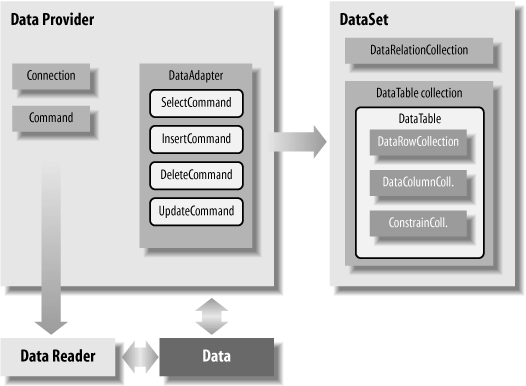
\includegraphics[width=0.9\textwidth]{ado-dot-net-architecture}
	\caption{ADO .\ NET Architecture.}\label{fig:ado-dot-net-objects}
\end{figure}

\subsection{ADO .\ NET Architecture}
The ADO.NET architecture has two main parts:
\begin{enumerate}
	\item \texttt{DataProvider} (Connected Objects or Connection oriented objects)
	\item \texttt{DataSet} (Disconnected objects or Connection-less objects)
\end{enumerate}


\subsubsection{DataProvider}
\begin{itemize}
	\item The .\ NET framework Data Provider is component that has been explicitly designed for data manipulation
	and fast, forward-only, read-only access to data.
	\item .\ NET Framework data provider is used for connecting to a database, executing commands, and retrieving
	results.
	\item The Data Provider has four core objects:
	\begin{enumerate}
		\item \textbf{Connection}: Establishes a connection to a specific data source
		\item \textbf{Command}: Executes a command against a data source
		\item \textbf{DataReader}: Reads a stream of data from a data source
		\item \textbf{DataAdapter}: Populates a data set and resolves updates with the data source
	\end{enumerate}
\end{itemize}
An ADO .\ NET data provider is a software component that interacts with a data source. ADO .\ NET
data providers are analogous to ODBC drivers, JDBC drivers, and OLE DB providers.

\noindent \emph{\textbf{Note}: ODBC (Open Database Connectivity) is designed to provide access primarily to SQL data in a multi-
platform environment. OLE DB (Object Linking and Embedding Database) is designed to provide access to all
types of data in an OLE Component Object Model (COM) environment. OLE DB includes the SQL functionality
defined in ODBC but also defines interfaces suitable for gaining access to data other than SQL data.}


\paragraph*{Connection}
\begin{itemize}
	\item The Connection object is the first component of ADO .\ NET.
	\item The Connection objects provider connectivity to a data source.
	\item It establishes a connection to a specific data source.
	\item Connection object helps in accessing and manipulating a database.
	\item The base class for all Connection objects in the \texttt{DbConnection} class.
	\item Example: See Section \ref{sec:connection}.
\end{itemize}

\paragraph*{Command}
\begin{itemize}
	\item The Command object enables access to database commands to return data, modify data, run stored procedures, and send or retrieve parameter information.
	\item It executes a command against a data source. Exposes Parameters and can execute in the scope of a Transaction from a Connection.
	\item You can execute SQL queries to return data in a \texttt{DataSet} or a \texttt{DataReader} object.
	\item Command object performs the standard Select, Insert, Delete and Update T-SQL operations.
	\item The base class for all Command objects is the \texttt{DbCommand} class.
	\item Example: See Section \ref{sec:command}.
\end{itemize}

\paragraph*{DataReader}
\begin{itemize}
	\item The Data Reader provides a high-performance stream of data from the data source.
	\item It reads a forward-only, read-only stream of data from a data source.
	\item \texttt{DataReader} object works in connected model.
	\item The base class for all \texttt{DataReader} objects is the \texttt{DbDataReader} class.
	\item Example: See Section \ref{sec:data-reader}.
\end{itemize}

\paragraph*{DataAdapter}
\begin{itemize}
	\item The Data Adapter provides the bridge between the Data Set object and the data source.
	\item The Data Adapter uses command object to execute SQL commands at the data source to both load the Data Set with data and reconcile changes that were made to the data in the dataset back
	to the data source.
	\item It populates a \texttt{DataSet} and resolves updates with the data source.
	\item The base class for all \texttt{DataAdapter} objects is the \texttt{DbDataAdapter} class.
\end{itemize}

\noindent The following lists the data providers that are included in the .\ NET framework.

\begin{enumerate}
	\item SQL Server
		\begin{itemize}
			\item Provides data access for Microsoft SQL server.
			\item Uses the \texttt{System.Data.SqlClient} namespace.
		\end{itemize}
	\item OLEDB
		\begin{itemize}
			\item For data sources exposed by using OLEDB.
			\item Uses the \texttt{System.Data.OleDb} namespace
		\end{itemize}
	\item ODBC
		\begin{itemize}
			\item For data sources exposed by using ODBC.
			\item Uses the \texttt{System.Data.Odbc} namespace.
		\end{itemize}
	\item Oracle
	\begin{itemize}
		\item For Oracle data sources.
		\item Uses the \texttt{System.Data.OracleClient} namespace.
	\end{itemize}
\end{enumerate}
Following Code demonstration of binding \texttt{GridView} control using Connection Oriented Objects of ADO .\ Net.

\lstinputlisting[caption=Example of GridView control using connection oriented objects]{ConnectionOrientedADO.cs}

\subsubsection{DataSet}
\begin{itemize}
	\item The dataset represents a subset of the database. 
	\item The dataset is a memory-resident representation of data that provides consistent relational programming
	\item It does not have a continuous connection to the database. 
	\item To update the database a re-connection is required. 
	\item The dataset represents a complete set of data, including related tables, constraints, and relationship
	among the table.
	\item The \texttt{DataSet} contains:
	\begin{enumerate}
		\item \texttt{DataTable} objects and 
		\item \texttt{DataRelation} objects. 
	\end{enumerate}

\end{itemize}

\paragraph*{DataRelation}
\begin{itemize}
	\item The \texttt{DataRelation} objects	represent the relationship between two tables.
	\item A relationship represented by the Data relation object, associated rows in one Data table with rows in another Data table.
	\item A relationship is analogous to a join path that might exist between primary and foreign key columns in a relational database.
	\item A data relation identifies matching columns in two tables of a dataset.
	\item The essential element of a data relation are:
		\begin{itemize}
			\item The name of the relationship
			\item The name of the tables being related
			\item The related column in each table
		\end{itemize}
	\item Relationship can be built with more than one column per table by specifying an array of Data Column objects as the key columns.
	\item Optionally, a Unique key constraint can be added to enforce integrity constraints when changes are made to related column values.
\end{itemize}


\noindent Listing \ref{lst:disconnected-objects-example} example demonstrate disconnected objects.

\lstinputlisting[label={lst:disconnected-objects-example}, caption=Example of disconnected objects]{DisconnectedADO.cs}


\paragraph*{DataTable}
\begin{itemize}
	\item The \texttt{DataTable} class represents the tables in the database. 
	\item A Data table is defined in the \texttt{System.Data} namespace and represents a single table of memory-resident data.
	\item It has the important properties as shown in Table \ref{tab:data-table-prop}; most of these properties are read only properties except the \texttt{PrimaryKey} property.
\end{itemize}


\begin{table}[ht!]
\centering	
	\caption{DataTable properites}\label{tab:data-table-prop}
\begin{tabular}{p{3cm}p{9cm}}
	\toprule
	\textbf{Properties}    & \textbf{Description}                                              \\ \midrule
	\verb|ChildRelations|  & Returns the collection of child relationship                      \\
	\verb|Columns|         & Returns the Columns collection                                    \\
	\verb|Constraints|     & Returns the Constraints collection                                \\
	\verb|DataSet|         & Returns the parent \texttt{DataSet}                                        \\
	\verb|DefaultView|     & Returns a view of the table                                       \\
	\verb|ParentRelations| & Returns the \texttt{ParentRelations} collection                            \\
	\verb|PrimaryKey|      & Gets or sets an array of columns as the primary key for the table \\
	\verb|Rows|            & Returns the Rows collection                                       \\ \bottomrule
\end{tabular}
\end{table}

\subparagraph*{DataRow}
The \texttt{DataRow} object represents a row in a table. It has the important properties as shown in Table \ref{tab:data-row-prop}:

\begin{table}[ht!]
	\centering
	\caption{DataRow properites}\label{tab:data-row-prop}
\begin{tabular}{p{3cm}p{9cm}}
	\toprule
	\textbf{Properties} & \textbf{Description}                                         \\ \midrule
	\texttt{HasErrors}  & Indicates if there are any errors relationship               \\
	\texttt{Items}      & Gets or sets the data stored in a specific column collection \\
	\texttt{ItemArrays} & Gets or sets all the values for the row                      \\
	\texttt{Table}      & Returns the parent table                                     \\ \bottomrule
\end{tabular}
\end{table}



%\subsubsection*{The DataAdapter Object}
%The DataAdapter object acts as a mediator between the DataSet object and the database. This helps the Dataset
%to contain data from multiple databases or other data source.
%
%\subsubsection*{The DataReader Object}
%The DataReader object is an alternative to the DataSet and DataAdapter combination. This object provides a
%connection oriented access to the data records in the database. These objects are suitable for read-only access,
%such as populating a list and then breaking the connection. \par 
%
%DataReader is read-only and forward only, meaning
%once you read a record and go to the next record, there is no way to go back to the previous record. It is also
%not possible to change the data using DataReader. DataReader is connection oriented, meaning it requires an
%active connection to the data source, while reading data. The forward-only nature of DataReader is what makes
%it an efficient choice to read data.

%\subsubsection*{DbCommand and DbConnection Objects}
%The \verb|DbConnection| object represents a connection to the data source. The connection could be shared among
%different command objects.
%\par
%
%The \verb|DbCommand| object represents the command or a stored procedure sent to the database for retrieving or
%manipulating data. \par

\section{Working with Connection, Command, DataReader}
An application needs to perform following steps to retrieve data from database:
\begin{enumerate}
\item  \textit{Connect to the Database}
\item  \textit{Prepare an SQL Command}
\item  \textit{Execute the Command}
\item  \textit{Retrieve the results and display in the application}
\end{enumerate}

\begin{itemize}
	\item The combination of \texttt{Connection}, \texttt{Command} and \texttt{DataReader} object gives us connected approach of
	connecting to database.
	\item Notice that we are using \texttt{SQLConnection}, \texttt{SQLCommand} and \texttt{SQLDataReader} classes. All the objects
	are prefixed with the word SQL. All these classes are present in \verb|System.Data.SqlClient| namespace. So,
	we can say that the .NET data provider for SQL Server is \verb|System.Data.SqlClient|.
	\item Sample ADO .\ NET code to connect to SQL Server Database and retrieve data using connection, command and \texttt{DataReader}:

	\lstinputlisting[caption={Example to connect sql server database and retrieve data using connection, command and reader}]{DbConnectionExample.cs}
	
	\item Sample ADO .\ NET code to connect to Oracle Database and retrieve data using connection, command and \texttt{DataReader}:
	
\begin{lstlisting}
	OracleConnection con = new OracleConnection("Oracle db Connection String");
	OracleCommand cmd = new OracleCommand("Select * from tblProduct", con);
	con.Open();
	OracleDataReader rdr = cmd.ExecuteReader();
	GridView1.DataSource = rdr;
	GridView1.DataBind();
	con.Close();
\end{lstlisting}
	Notice that we are using \texttt{OracleConnection}, \texttt{OracleCommand} and \texttt{OracleDataReader} classes. All the
objects are prefixed with the word Oracle. All these classes are present in \texttt{System.Data.OracleClient}
namespace. So, we can say that the .\ NET data provider for Oracle is \texttt{System.Data.OracleClient}.

\item Another example of using \texttt{DataReader} to load data:

\lstinputlisting[caption= {DataReader example}]{data-reader-example-2.cs}

If for some reason, you want to loop through each row in the \texttt{SqlDataReader} object, then use
the \texttt{Read()} method, which returns true as long as there are rows to read. If there are no more rows to
read, then this method will return false. In the following example, we loop through each row in
the \texttt{SqlDataReader} and then compute the 10\% discounted price.

\end{itemize}


\emph{If we want to connect to OLEDB datasources like Excel, Access etc, we can use OleDbConnection, OleDbCommand and OleDbDataReader classes. So, \. NET data provider for OLEDB is \texttt{System.Data.OleDb}.}

\subsubsection*{Different .NET Data Providers}
\begin{itemize}
	\item Data Provider for SQL Server - \texttt{System.Data.SqlClient}
	\item Data Provider for Oracle - \texttt{System.Data.OracleClient}
	\item Data Provider for OLEDB - \texttt{System.Data.OleDb}
	\item Data Provider for ODBC - \texttt{System.Data.Odbc}
\end{itemize}


Depending on the provider, the following ADO .\ NET objects have a different prefix:
\begin{multicols}{2}
		\begin{enumerate}
		\item \textit{Connection}: 
		\begin{itemize}
			\item \texttt{SQLConnection}, 
			\item \texttt{OracleConnection}, 
			\item \texttt{OleDbConnection}, 
			\item \texttt{OdbcConnection}, etc.
		\end{itemize}
	
		\item \textit{Command}: 
		\begin{itemize}
			\item \texttt{SQLCommand}, 
			\item \texttt{OracleCommand}, 
			\item \texttt{OleDbCommand}, 
			\item \texttt{OdbcCommand}, etc.
		\end{itemize}
	\item \textit{DataReader}: 
		\begin{itemize}
			\item \texttt{SQLDataReader}, 
			\item \texttt{OracleDataReader}, 
			\item \texttt{OleDbDataReader}, 
			\item \texttt{OdbcDataReader}, etc.
		\end{itemize}

		\item \textit{DataAdapter}: 
		\begin{itemize}
			\item \texttt{SQLDataAdapter}, 
			\item \texttt{OracleDataAdapter}, 
			\item \texttt{OleDbDataAdapter}, 
			\item \texttt{OdbcDataAdapter}, etc.
		\end{itemize}
	\end{enumerate}
\end{multicols}


\subsection{Connection}\label{sec:connection}
\begin{itemize}
	\item It is used to establish an open connection to the SQL Server database. 
	\item It is a sealed class. So, it cannot be inherited. 
	\item \texttt{SqlConnection} class uses \texttt{SqlDataAdapter} and \texttt{SqlCommand} classes together to increase performance when connecting to a Microsoft SQL Server database.
	\item Connection does not close explicitly even it goes out of scope. Therefore, you must explicitly close the connection by calling \texttt{Close()} method.	
	\item \texttt{Using} block is used to close the connection automatically. 
	\item We don't need to call \texttt{Close()} method explicitly, \texttt{Using} block do this for ours program implicitly when the code exits the block.
\end{itemize}

\subsubsection*{Example}
\begin{lstlisting}
using (SqlConnection con = new SqlConnection(connectionString)) {    
	con.Open();         
} 
\end{lstlisting}



\lstinputlisting[caption={Example of sqlConnection}]{sqlConnectionExample.cs}

\subsection{Command}\label{sec:command}
\begin{itemize}
	\item This class is used to store and execute SQL statement for SQL Server database. 
	\item It is a sealed class. So, it cannot be inherited.
\end{itemize}

\subsubsection*{Example}
\lstinputlisting[caption={Example of sqlCommand}]{sqlCommandExample.cs}



\subsection{DataReader}\label{sec:data-reader}
\begin{itemize}
	\item This class is used to read data from SQL Server database. 
	\item It reads data in forward-only stream of rows from a SQL Server database. 
	\item It is sealed class so that cannot be inherited. 
	\item It inherits \texttt{DbDataReader} class and implements \texttt{IDisposable} interface.
\end{itemize}



\lstinputlisting[caption={Example of sqlDataReaderExample.}]{sqlDataReaderExample.cs}


\section{Working With Dataset}
\begin{itemize}
	\item The ADO .\ NET \texttt{DataSet} is a memory-resident representation of data that provides a consistent relational
	programming model regardless of the source of the data it contains. 
	\item A \texttt{DataSet} represents a complete set of data including the tables that contain, order, and constrain the data, as well as the relationships
	between the tables.
	\item There are several ways of working with a DataSet, which can be applied independently or in combination.
	 We can:
	 \begin{itemize}
	 	\item Programmatically create a \texttt{DataTable}, \texttt{DataRelation}, and Constraint within a \texttt{DataSet} and populate the tables with data.
	 	\item Populate the \texttt{DataSet} with tables of data from an existing relational data source using a \texttt{DataAdapter}.
	 	\item Load and persist the \texttt{DataSet} contents using \texttt{XML}.
	 \end{itemize}
\end{itemize}


\subsection*{Creating DataSet Programatically}
\begin{itemize}
	\item In this program, we create two \texttt{DataTables}. 
	\item One stores two rows of patient information. 
	\item And the second stores two rows of medication information.
	\item We create a \texttt{DataSet} with the \texttt{DataSet} constructor. 
	\item Then we add the two \texttt{DataTables} to the \texttt{DataSet} instance. 
	\item Finally we print the \texttt{XML}.
\end{itemize}

\lstinputlisting[caption={Creating DataSet}, label={lst:dataset-example}]{dataset-example.cs}

\lstinputlisting[language=xml, caption={Output from Listing \ref{lst:dataset-example}}]{dataSetOutput.xml}


\subsection*{Populating DataSet with tables from database}
\begin{itemize}
	\item Following program send query to stored procedure in database and loads the table data into dataset. 
	\item The stored procedure for this would be:
\end{itemize}


\begin{lstlisting}[language=sql]
Create procedure spGetProductAndCategoriesData
as
	Begin
	Select ProductId, ProductName, UnitPrice
	from tblProductInventory
	Select CategoryId, CategoryName
	from tblProductCategories
End
\end{lstlisting}

And the program is illustrated in Listing \ref{lst:populate-dataset-database} calls stored procedure and loads data into dataset.

\begin{lstlisting}[caption={Loading data into DataSet using}, label={lst:populate-dataset-database}]
string ConnectionString = ConfigurationManager.ConnectionStrings["DBConnectionString"].ConnectionString;
using(SqlConnection connection = new SqlConnection(ConnectionString)) {
	SqlDataAdapter dataAdapter = new SqlDataAdapter("spGetProductAndCategoriesData", connection);
	dataAdapter.SelectCommand.CommandType = CommandType.StoredProcedure;
	DataSet dataset = new DataSet();
	dataAdapter.Fill(dataset);
	GridViewProducts.DataSource = dataset.Tables[0];
	GridViewProducts.DataBind();
	GridViewCategories.DataSource = dataset.Tables[1];
	GridViewCategories.DataBind();
}
\end{lstlisting}

\section{Adding, Deleting and Modifying Records in Dataset}
You edit data in data tables (\texttt{DataSet}) much like you edit the data in a table in any database. The process can include
inserting, updating, and deleting records in the table.

\subsection*{Editing/Modifying records:}
To edit an existing row in a \texttt{DataTable}, you need to locate the \texttt{DataRow} you want to edit, and then assign the updated
values to the desired columns. If you don't know the index of the row you want to edit, use the \texttt{FindBy} method to search
by the primary key.

\subsection*{Adding records:}
To add new records to a dataset, create a new data row by calling the method on the \texttt{DataTable}. Then add the row to
the \texttt{DataRow} collection (Rows) of the \texttt{DataTable}.

\subsection*{Deleting records:}
Call the Delete method of a DataRow.

\subsection*{Example}
\lstinputlisting[caption=CRUD operation in dataset]{dataset-crud.cs}


\section{Using DataView}
\begin{itemize}
	\item A \texttt{DataView} enables you to create different views of the data stored in a \texttt{DataTable}, a capability that is often used
	in data-binding applications. 
	\item Using a \texttt{DataView}, you can expose the data in a table with different sort orders, and	you can filter the data by row state or based on a filter expression.
	\item A \texttt{DataView} provides a dynamic view of data in the underlying \texttt{DataTable}: 
	\begin{itemize}
		\item the content, ordering, and membership reflect changes as they occur. 
	\end{itemize}
	\item This behavior differs from the Select method of the \texttt{DataTable}, which returns a \texttt{DataRow} array from a table based on a particular filter and/or sort order:
\begin{itemize}
	\item this content reflects changes to the underlying table, but its membership and ordering remain static. 
\end{itemize}
	\item The dynamic capabilities of the \texttt{DataView} make it ideal for data-binding applications.
	\item A \texttt{DataView} provides you with a dynamic view of a single set of data, much like a database view, to which you can apply different sorting and filtering criteria. Unlike a database view, however, a \texttt{DataView} cannot be treated as a table and cannot provide a view of joined tables. You also cannot exclude columns that exist in the source table, nor can you append columns, such as computational columns, that do not exist in the source table.
	
	\item You can use a \texttt{DataViewManager} to manage view settings for all the tables in a \texttt{DataSet}. 
	\item The \texttt{DataViewManager} provides you with a convenient way to manage default view settings for each table. When binding a control to more than one table of a \texttt{DataSet}, binding to a \texttt{DataViewManager} is the ideal choice.
\end{itemize}




\subsection*{Creating DataView}
There are two ways to create a \texttt{DataView}. You can use the \texttt{DataView} constructor, or you can create a reference
to the \texttt{DefaultView} property of the DataTable. The \texttt{DataView} constructor can be empty, or it can take either a
\texttt{DataTable} as a single argument, or a \texttt{DataTable} along with filter criteria, sort criteria, and a row state filter.

The following code example demonstrates how to create a \texttt{DataView} using the \texttt{DataView} constructor. A \texttt{RowFilter},
\texttt{Sort} column, and \texttt{DataViewRowState} are supplied along with the \texttt{DataTable}.


\begin{lstlisting}
DataView custDV = new DataView(custDS.Tables["Customers"], "Country = 'Nepal'", "ContactName", DataViewRowState.CurrentRows);
\end{lstlisting}

The following code example demonstrates how to obtain a reference to the default DataView of a DataTable using the DefaultView property of the table.
\begin{lstlisting}
DataView custDV = custDS.Tables["Customers"].DefaultView;
\end{lstlisting}

\subsubsection*{Example of DataView}
\lstinputlisting[caption={Example of DataView}]{DataView.cs}

\section{Working With DataGridVeiw}
DataGridView displays data from SQL databases. This example takes a specific table from a database and display
it on a DataGridView. This is done with a DataAdapter and data table. A visual representation of data is the end
result.

\begin{lstlisting}[caption=Working with DataGridView.]
void FillData() {
	// 1 Open connection
	using(SqlConnection c = new SqlConnection( Properties.Settings.Default.DataConnectionString)) {
		c.Open(); 
		
		// 2 Create new DataAdapter
		using(SqlDataAdapter a = new SqlDataAdapter( "SELECT * FROM Animals", c)) {
			// 3 Use DataAdapter to fill DataTable
			DataTable t = new DataTable();
			a.Fill(t);
			
			// 4  Render data onto the screen
			dataGridView1.DataSource = t;
		}
	}
}
\end{lstlisting}

\subsubsection*{Example of DataGridView}
\lstinputlisting[caption={Example of DataGridView CRUD}]{DataGridViewCRUD.cs}

\section{Calling Stored procedure}

First, create the following stored procedure in MSSQL Server.
\begin{lstlisting}[caption= {Stored procedure}, language=sql]
Create procedure spGetProductAndCategoriesData
as
Begin
	Select ProductId, ProductName, UnitPrice
	from tblProductInventory
	Select CategoryId, CategoryName
	from tblProductCategories
End
\end{lstlisting}

And the program below calls stored procedure and loads data into dataset.
\lstinputlisting[caption=Calling stored procedure]{calling-stored-procedure.cs}

\newpage\thispagestyle{empty} % ch-6: Data Access with ADO .\ NET
\chapter{Web Application}

\section{Basic Concepts of Web Application Development}
%https://en.wikipedia.org/wiki/Web_application
A web application (or web app) is application software that runs on a web server, unlike software programs that are run locally on the operating system (OS) of the device. Web applications are accessed by the user through a web browser with an active internet connection. These applications are programmed using a client–server modeled structure—the user (``client") is provided services through an off-site server that is hosted by a third party. Examples of commonly-used web applications include: web-mail, online retail sales, online banking, and online auctions.

%https://www.staticapps.org/articles/defining-static-web-apps/
A Static Web Application is any web application that can be delivered directly to an end user's browser without any server-side alteration of the HTML, CSS, or JavaScript content. While this can encompass very flat, unchanging sites like a corporate web site, static web applications generally refer to rich sites that utilize technologies in the browser instead of on the server to deliver dynamic content.

%https://stackoverflow.com/questions/42735947/difference-between-a-dynamic-web-application-and-a-normal-web-application#:~:text=A%20dynamic%20web%20application%20generates,when%20you%20click%20on%20follow.
A dynamic web application generates the pages/data in real time, as per the request, a respective response will trigger from the server end and will reach the client end. Depending upon the response the client side code will take action as it's supposed to.



\section{Implementing Session and Cookies}
\subsection{Cookies}
A cookie is a token that the Web server embeds in a user's Web browser to identify the user. The next time the same browser requests a page, it sends the cookie it received from the Web server. Cookies allow a set of information to be associated with a user. ASP scripts can both get and set the values of cookies by using the \texttt{Response.Cookies} {Collection collection} of the \textbf{Response} and \textbf{Request} objects. Once a cookie has been set, all page requests that follow return the cookie name and value. A cookie can only be read from the domain that it has been issued from. If a cookie contains a collection of multiple values, we say that the cookie has Keys.

\noindent Note: \emph{The maximum cookie size is 4KB.}

\subsubsection{Types of  Cookies}
\begin{enumerate}
	\item \textbf{Persistence Cookie}: Has an expiry time.
	\item \textbf{Non-Persistence Cookie}: Maintains user information as long as the user accesses the same browser. It will be discarded when user closes the browser.
\end{enumerate}

\subsubsection{Set/Create Cookies}
\begin{itemize}
	\item To set the value of a cookie, use \verb*|Response.Cookies|
	\item If the cookie does not already exist, \verb*|Response.Cookies| creates a new one
	\item Cookie can have multiple values; such a cookie is called an indexed cookie.
	\item The \verb*|Response.Cookies| command must appear before the \verb*|<html>| tag.
\begin{lstlisting}
<%
	// create a cookie named 'semester' with the value '8'
	Response.Cookies("semester")= 8
	
	// create a cookie named 'name' with the value 'Jeevan'
	Response.Cookies("name")="Jeevan"
	
	// assign 'Expires' property to a cookie
	Response.Cookies("name").Expires= "Jan 20,2021"
%>
\end{lstlisting}

\subsubsection*{A Cookie with Keys}
\begin{lstlisting}
<%
	/* create a cookie collection named 'student' */
	Response.Cookies("student")("firstname")="Jeevan"
	Response.Cookies("student")("lastname")="P"
	Response.Cookies("student")("district")="Taplejung"
%>
\end{lstlisting}

\end{itemize}

\subsubsection{Get/Retrieve Cookies}
\begin{itemize}
\item The \verb*|Request.Cookies| command is used to retrieve a cookie value
\item In the example below, we retrieve the value of the cookie named `name' and display it on a page:
\begin{lstlisting}
<%
	name=Request.Cookies("name")
	response.write("Name=" & name)
	// output: Name=Jeevan
%>
\end{lstlisting}

\lstinputlisting[caption=Reading all cookies]{CookiesExample.aspx}

\end{itemize}


\subsection{Session}
The web server does not know who you are and what you do, because the HTTP address doesn't maintain state. 


ASP solves this problem by creating a unique cookie for each user. The cookie is sent to the user's computer and it contains information that identifies the user. This interface is called the Session object. 

The Session object stores information about, or change settings for a user session.

Variables stored in a Session object hold information about one single user, and are available to all pages in one application. Common information stored in session variables are name, id, and preferences. The server creates a new Session object for each new user, and destroys the Session object when the session expires.

A session starts when:

\begin{itemize}
	\item A new user requests an ASP file, and the Global.asa file includes a \verb*|Session_OnStart| procedure
	\item A value is stored in a Session variable
	\item A user requests an ASP file, and the \verb*|Global.asa| file uses the \verb*|<object>| tag to instantiate an object with session scope
\end{itemize}
A session ends if a user has not requested or refreshed a page in the application for a specified period. By default, this is 20 minutes.

If you want to set a timeout interval that is shorter or longer than the default, use the Timeout property.

The example below sets a timeout interval of 5 minutes:

\begin{lstlisting}
<%
	Session.Timeout=5
%>
\end{lstlisting}

Use the \verb*|Abandon| method to end a session immediately:
\begin{lstlisting}
<%
	Session.Abandon
%>
\end{lstlisting}

Note: The main problem with sessions is WHEN they should end. We do not know if the user's last request was the final one or not. So we do not know how long we should keep the session ``alive". Waiting too long for an idle session uses up resources on the server, but if the session is deleted too soon the user has to start all over again because the server has deleted all the information. Finding the right timeout interval can be difficult!

\subsubsection*{Store and Retrieve Session Variables }
The most important thing about the Session object is that you can store variables in it.

The example below will set the Session variable username to ``Donald Duck" and the Session variable age to ``50":
\begin{lstlisting}
<%
	Session("username")="Donald Duck"
	Session("age")=50
%>
\end{lstlisting}
When the value is stored in a session variable it can be reached from ANY page in the ASP application:
\begin{lstlisting}
Welcome <%Response.Write(Session("username"))%>
\end{lstlisting}

The line above returns: ``Welcome Donald Duck".

You can also store user preferences in the Session object, and then access that preference to choose what page to return to the user.

The example below specifies a text-only version of the page if the user has a low screen resolution: 
\begin{lstlisting}
<%If Session("screenres")="low" Then%>
	This is the text version of the page
<%Else%>
	This is the multimedia version of the page
<%End If%>
\end{lstlisting}

\subsubsection*{Remove Session Variables }
The Contents collection contains all session variables.

It is possible to remove a session variable with the Remove method.

The example below removes the session variable ``sale" if the value of the session variable ``age" is lower than 18: 
\begin{lstlisting}
<%
If Session.Contents("age")<18 then
	Session.Contents.Remove("sale")
End If
%>
\end{lstlisting}

To remove all variables in a session, use the RemoveAll method: 
\begin{lstlisting}
<%
	Session.Contents.RemoveAll()
%>
\end{lstlisting}

\subsubsection*{Loop Through The Contents Collection}
The Contents collection contains all session variables. You can loop through the Contents collection, to see what's stored in it:
\begin{lstlisting}
<%
	Session("username")="Donald Duck"
	Session("age")=50
	
	dim i
	For Each i in Session.Contents
	Response.Write(i & "<br>")
	Next
	
	/*  output: 
		username
		age 
	*/
%>
\end{lstlisting}
If you do not know the number of items in the Contents collection, you can use the Count property:
\begin{lstlisting}
<%
	dim i
	dim j
	j=Session.Contents.Count
	Response.Write("Session variables: " & j)
	For i=1 to j
	Response.Write(Session.Contents(i) & "<br>")
	Next
	
	/* output:
		Session variables: 2
		Donald Duck
		50
	*/	
%>
\end{lstlisting}

\subsubsection*{Loop Through The StaticObjects Collection}
You can loop through the StaticObjects collection, to see the values of all objects stored in the Session object:
\begin{lstlisting}
<%
	dim i
	For Each i in Session.StaticObjects
	Response.Write(i & "<br>")
	Next
%>
\end{lstlisting}
\section{Client and Server Side Validation}
Validation is a set of rules that you apply to the data you collect.
These rules can be many or few and enforced either strictly or in a lax manner: It really depends
on you. No perfect validation process exists because some users may find a way cheat to some
degree, no matter what rules you establish. The trick is to find the right balance of the fewest rules
and the proper strictness, without compromising the usability of the application. 

The data you collect for validation comes from the Web forms you provide in your applications.
Web forms are made up of different types of HTML elements that are constructed using raw
HTML form elements, ASP .\ NET HTML server controls, or ASP .\ NET Web Form server controls. In the end, your forms are made up of many types of HTML elements, such as text boxes, radio
buttons, check boxes, drop-down lists, and more.

\subsection{Client Side Validation}
Client-side validation is quick and responsive for the end user. It is something end users expect of the
forms that they work with. If something is wrong with the form, using client-side validation ensures that
the end user knows this as soon as possible. Client-side validation also pushes the processing power
required of validation to the client meaning that you don’t need to spin CPU cycles on the server to process the same information because the client can do the work for you.

With this said, client-side validation is the more insecure form of validation. When a page is generated in
an end user’s browser, this end user can look at the code of the page quite easily (simply by right-clicking
his mouse in the browser and selecting View Code). When he does this, in addition to seeing the HTML
code for the page, he can also see all the JavaScript that is associated with the page. If you are validating
your form client-side, it doesn’t take much for the crafty hacker to repost a form (containing the values he wants in it) to your server as valid. There are also the cases in which clients have simply disabled the
client-scripting capabilities in their browsers - thereby making your validations useless. Therefore,
client-side validation should be looked on as a convenience and a courtesy to the end user and never as
a security mechanism


\subsection{Server Side Validation}
The more secure form of validation is server-side validation. Server-side validation means that the validation checks are performed on the server instead of on the client. It is more secure because these checks cannot be easily bypassed. Instead, the form data values are checked using server code ({\cs} or VB) on the server. If the form isn’t valid, the page is posted back to the client as invalid. Although it is more secure,
server-side validation can be slow. It is sluggish simply because the page has to be posted to a remote
location and checked. Your end user might not be the happiest surfer in the world if, after waiting 20
seconds for a form to post, he is told his e-mail address isn’t in the correct format.

The best approach is always to perform client-side validation first and then, after the form passes and is posted to the server, to perform the validation checks
again using server-side validation This approach provides the best of both worlds. It is secure because
hackers can’t simply bypass the validation. They may bypass the client-side validation, but they quickly
find that their form data is checked once again on the server after it is posted. 

\subsection{ASP .\ NET Validation Server Controls}
In the classic ASP days, developers could spend a great deal of their time dealing with different form
validation schemes. For this reason, with the initial release of ASP .\ NET, the ASP .\ NET team introduced a
series of validation server controls meant to make it a snap to implement sound validation for forms.

ASP .\ NET not only introduces form validations as server controls, but it also makes these controls rather
smart. As stated earlier, one of the tasks of classic ASP developers was to determine where to perform
form validation — either on the client or on the server. The ASP .\ NET validation server controls eliminate
this dilemma because ASP .\ NET performs browser detection when generating the ASP .\ NET page and
makes decisions based on the information it gleans.

This means that if the browser can support the JavaScript that ASP .\ NET can send its way, the validation
occurs on the client-side. If the client cannot support the JavaScript meant for client-side validation, this
JavaScript is omitted and the validation occurs on the server.

The best part about this scenario is that even if client-side validation is initiated on a page, ASP .\ NET still
performs the server-side validation when it receives the submitted page, thereby ensuring security won’t
be compromised. This decisive nature of the validation server controls means that you can build your
ASP .\ NET Web pages to be the best they can possibly be.

The available validation controls include:

\begin{multicols}{2}
	\begin{enumerate}
		\item RequiredFieldValidator
		\item CompareValidator
		\item RangeValidator
		\item RegularExpressionValidator
		\item CustomValidator
		\item ValidationSummary
	\end{enumerate}
\end{multicols}


The Table \ref{tab:validation-server-control} describes the functionality of each of the available validation server controls.


\begin{table}[ht!]
	\centering
	\caption{Validation Server Controls.}\label{tab:validation-server-control}
\begin{tabular}{p{5cm}p{7cm}}
	\toprule
	\textbf{Validation Server Control} & \textbf{Description} \\
	\midrule
	
	\texttt{RequiredFieldValidator} 		& Ensures that the user does not skip a form entry field\\
	
	\texttt{CompareValidator}			& Allows for comparisons between the user’s input and another item using a comparison operator (equals, greater than, less than, and so on)\\
	
	\texttt{RangeValidator}				& Checks the user’s input based upon a lower- and upper level range of numbers or characters\\
	
	\texttt{RegularExpressionValidator} 	& Checks that the user’s entry matches a pattern defined by a regular expression. This is a good control to use to check e-mail addresses and phone numbers \\
	
	\texttt{CustomValidator} 			& Checks the user's entry using custom-coded validation logic\\
	\texttt{ValidationSummary}			& Displays all the error messages from the validators in one specific spot on the page\\
	\bottomrule	
\end{tabular}
\end{table}


\subsubsection{The RequiredFieldValidator Server Control}
\begin{itemize}
	\item The \texttt{RequiredFieldValidator} control simply checks to see if something was entered into the HTML form
	element. 
	\item It is a simple validation control, but it is one of the most frequently used. 
	\item You must have a \texttt{RequiredFieldValidator} control for each form element on which you wish to enforce a \textit{value-required} rule.
	
\end{itemize}

\paragraph*{VB} Listing \ref{lst:required-field-validate} shows a simple use of the \texttt{RequiredFieldValidator} server control using VB.

\lstinputlisting[style=vb, label={lst:required-field-validate}, caption=A simple use of the RequiredFieldValidator server control using VB.]{required-field-validate.aspx}

\paragraph*{\cs}
Listing \ref{lst:required-field-validate-cs} shows a simple use of the \texttt{RequiredFieldValidator} server control using \cs.
\lstinputlisting[label={lst:required-field-validate-cs}, caption= A simple use of the RequiredFieldValidator server control using \cs.]{required-field-validate-cs.aspx}


\subsubsection{The CompareValidator Server Control}
\begin{itemize}
	\item The \texttt{CompareValidator} control allows you to make comparisons between two form elements as well as
	to compare values contained within form elements to constants that you specify. 
	\item For instance, you can	specify that a form element’s value must be an integer and greater than a specified number. 
	\item You can also state that values must be strings, dates, or other data types that are at your disposal.
\end{itemize}

\paragraph*{VB}
Listing \ref{lst:compare-validator-vb} shows the use of \texttt{CompareValidator}.

\lstinputlisting[style=vb, caption=Using the CompareValidator to test values against other control values, label={lst:compare-validator-vb}]{compare-validator-vb.aspx}

\paragraph*{\cs}

Listing \ref{lst:compare-validator-cs} shows the use of \texttt{CompareValidator} with \cs.
\lstinputlisting[caption=Using the CompareValidator to test values against other control values with \cs, label={lst:compare-validator-cs}]{compare-validator-cs.aspx}

\subsubsection{The RangeValidator Server Control}
\begin{itemize}
	\item The \texttt{RangeValidator} control is quite similar to that of the \texttt{CompareValidator} control, but it makes sure
	that the end user value or selection provided is between a specified range as opposed to being just	greater than or less than a specified constant. 
	\item For an example of this, go back to the text-box element that asks for the age of the end user and performs a validation on the value provided.
\end{itemize}

\begin{lstlisting}[numbers=none, caption=Using the RangeValidator control to test an integer value.]
Age:
<asp:TextBox ID="TextBox1" Runat="server"></asp:TextBox>
&nbsp;
<asp:RangeValidator ID="RangeValidator1" Runat="server"
ControlToValidate="TextBox1" Type="Integer"
ErrorMessage="You must be between 30 and 40"
MaximumValue="40" MinimumValue="30"></asp:RangeValidator>
\end{lstlisting}

\paragraph*{VB}
Listing \ref{lst:range-valid-date-vb} shows the use of \texttt{RangeValidator} control to test a string date value with VB.


\lstinputlisting[style=vb, caption=Using the RangeValidator control to test a string date value with VB, label={lst:range-valid-date-vb}]{range-validator-date-vb.aspx}


\paragraph*{\cs}
Listing \ref{lst:range-valid-date-cs} shows the use of \texttt{RangeValidator} control to test a string date value with \cs.
\lstinputlisting[caption=Using the RangeValidator control to test a string date value with \cs, label={lst:range-valid-date-cs}]{range-validator-date-cs.aspx}

\subsubsection{The RegularExpressionValidator Server Control}
\begin{itemize}
	\item This control offers a lot of flexibility when you apply validation rules to your Web forms. 
	\item Using the	\texttt{RegularExpressionValidator} control, you can check a user’s input based on a pattern that you define
	using a regular expression.
	\item This means that you can define a structure that a user’s input will be applied against to see if its structure matches the one that you define. \item For instance, you can define that the structure of the user input must be in the form of an e-mail address or an Internet \texttt{URL}; if it doesn't match this definition, the page
	is considered invalid.
\end{itemize}

Listing {\ref{lst:regex-valid-email}} shows how to validate what is input into a text box by making sure it is in the form of an e-mail address.

\lstinputlisting[caption=Making sure the text-box value is an e-mail address, label={lst:regex-valid-email}]{regex-valid-email.aspx}

Just like the other validation server controls, the \texttt{RegularExpressionValidator} control uses the
\texttt{ControlToValidate} property to bind itself to the \texttt{TextBox} control, and it includes an \texttt{ErrorMessage}
property to push out the error message to the screen if the validation test fails. The unique property of
this validation control is the \texttt{ValidationExpression} property. This property takes a string value,
which is the regular expression you are going to apply to the input value.

\subsubsection{The CustomValidator Server Control}
\begin{itemize}
	\item Validation controls described above are enough for us but if none of those works for us then we can use \textit{CustomValidator} control.
	 \item The \texttt{CustomValidator} control allows you to build your own client-side or server-side validations that can then be easily applied to your Web forms. 
	 \item Doing so allows you to make validation checks against values or calculations performed in the data tier (for example, in a database), or to make sure that the user's input validates against some arithmetic validation (for example, determining if a number is even or odd).
\end{itemize}


\paragraph*{Using Client Side Validation}
\begin{itemize}
	\item One of the worthwhile functions of the \texttt{CustomValidator} control is its capability to easily provide custom client-side validations. 
	
	\item Many developers have their own collections of JavaScript functions they employ in their applications, and using the \texttt{CustomValidator} control is one easy way of getting these functions implemented.
	
	\item For example, look at a simple form that asks for a number from the end user. 
	\item This form uses the \texttt{CustomValidator} control to perform a custom client-side validation on the user input to make sure that the number provided is divisible by 5. 
	\item This is illustrated in Listing {\ref{lst:custom-validator-client-vb}}.
	
\end{itemize}

\subparagraph*{VB}
Listing {\ref{lst:custom-validator-client-vb}} illustrates the CustomValidator control to perform client-side validations with VB.

\lstinputlisting[
	style=vb, 
	caption={Using the CustomValidator control to perform client-side validations with VB.}, label={lst:custom-validator-client-vb}
]{custom-validator-client-vb.aspx}

\subparagraph*{\cs}
Listing {\ref{lst:custom-validator-client-cs}} illustrates the CustomValidator control to perform client-side validations with \cs.

\lstinputlisting[
	caption={Using the CustomValidator control to perform client-side validations with \cs.}, label={lst:custom-validator-client-cs}
]{custom-validator-client-cs.aspx}

Looking over this Web form, you can see a couple of things happening. First, it is a simple form with
only a single text box requiring user input. The user clicks the button that triggers the \texttt{Button1\_Click}
event that, in turn, populates the Label1 control on the page. It carries out this simple operation only if
all the validation checks are performed and the user input passes these tests.

\paragraph*{Using Server-Side Validation}
\begin{itemize}
	\item Now let’s move this same validation check from the client to the server. 
	\item The \texttt{CustomValidator} control allows you to make custom server-side validations a reality as well. 
	
	\item \texttt{CustomValidator} for server-side validations is something you do if you want to check the user’s input against dynamic values coming from XML files, databases, or elsewhere.
	
	\item For an example of using the \texttt{CustomValidator} control for some custom server-side validation, you can work with the same example as you did when creating the client-side validation. 
	\item Now, create a server-side check that makes sure a user-input number is divisible by 5. 
	\item This is illustrated in Listing {\ref{lst:custom-validator-server-vb}} and {\ref{lst:custom-validator-server-cs}}.
\end{itemize}


\subparagraph*{VB}
Using the CustomValidator control to perform server-side validations with VB.
\lstinputlisting[
style=vb,
caption={Using the CustomValidator control to perform server-side validations with VB.}, label={lst:custom-validator-server-vb}
]{custom-validator-server-vb.aspx}



\subparagraph*{{\cs}}
Using the CustomValidator control to perform server-side validations with \cs.
\lstinputlisting[
	caption={Using the CustomValidator control to perform server-side validations with \cs.}, label={lst:custom-validator-server-cs}
]{custom-validator-server-cs.aspx}

Instead of a client-side JavaScript function in the code, this example includes a server-side function — \texttt{ValidateNumber}. The \texttt{ValidateNumber} function, as well as all functions that are being constructed to
work with the \texttt{CustomValidator} control, must use the \texttt{ServerValidateEventArgs} object as one of the
parameters in order to get the data passed to the function for the validation check. The \texttt{ValidateNumber}
function itself is nothing fancy. It simply checks to see if the provided number is divisible by 5.

\subsubsection{The ValidationSummary Server Control}
\begin{itemize}
	\item The \texttt{ValidationSummary} control is not a control that performs validations on the content input into your Web forms. 
	\item Instead, this control is the reporting control, which is used by the other validation controls on a page. 
	\item You can use this validation control to consolidate error reporting for all the validation errors
	that occur on a page instead of leaving this up to each and every individual validation control.
	\item By default, the \texttt{ValidationSummary} control shows the list of validation errors as a bulleted list. 
	\item This is illustrated in Listing {\ref{lst:validation-summary}}.
\end{itemize}

\lstinputlisting[
language=html,
caption={A partial page example of the ValidationSummary control.}, label={lst:validation-summary}
]{validation-summary.aspx}

This example asks the end user for her first and last name. Each text box in the form has an associated
\texttt{RequiredFieldValidator} control assigned to it. When the page is built and run, if the user clicks the
Submit button with no values placed in either of the text boxes, it causes both validation errors to fire.

As in earlier examples of validation controls on the form, these validation errors appear next to each of
the text boxes. You can see, however, that the \texttt{ValidationSummary} control also displays the validation
errors as a bulleted list in red at the location of the control on the Web form. In most cases, you do not
want these errors to appear twice on a page for the end user.


\section{Building Web Application}
\subsection*{Hosting}

\subsection*{Internet Information Services (IIS)}
%Internet Information Services (IIS) is a flexible, general-purpose web server from Microsoft that runs on Windows systems to serve requested HTML pages or files.
%
%An IIS web server accepts requests from remote client computers and returns the appropriate response. This basic functionality allows web servers to share and deliver information across local area networks (LAN), such as corporate intranets, and wide area networks (WAN), such as the internet.
%
%A web server can deliver information to users in several forms, such as static webpages coded in HTML; through file exchanges as downloads and uploads; and text documents, image files and more.

Stands for “Internet Information Services”. IIS is a web server software package designed for Windows Server. It is used for hosting websites and other content on the Web.

Microsoft’s Internet Information Services provides a graphical user interface (GUI) for managing websites and the associated users. It provides a visual means of creating, configuring, and publishing sites on the web. The IIS Manager tool allows web administrators to modify website options, such as default pages, error pages, logging settings, security settings, and performance optimizations.

IIS can serve both standard HTML webpages and dynamic webpages, such as ASP .\ NET applications and PHP pages. When a visitor accesses a page on a static website, IIS simply sends the HTML and associated images to the user’s browser. When a page on a dynamic website is accessed, IIS runs any applications and processes any scripts contained in the page, then sends the resulting data to the user’s browser.

While IIS includes all the features necessary to host a website, it also supports extensions (or “modules”) that add extra functionality to the server. For example, the WinCache Extension enables PHP scripts to run faster by caching PHP processes. The URL Rewrite module allows webmasters to publish pages with friendly URLs that are easier for visitors to type and remember. A streaming extension can be installed to provide streaming media to website visitors.

IIS is a popular option for commercial websites, since it offers many advanced features and is supported by Microsoft. However, it also requires requires a commercial license and the pricing increases depending on the number of users. Therefore, Apache HTTP Server, which is open source and free for unlimited users, remains the most popular web server software.

\subsubsection*{Features of IIS}

\paragraph*{Application pools}
 Application pools form an important part of an IIS server system. An individual application pool could have zero or many IIS worker processes running. These worker processes are responsible for running application instances.



\paragraph*{Authentication}
IIS server features authentication options, including Windows auth, Basic, and ASP .\ NET. If you use Windows Active Directory, Windows auth is especially useful, because it lets you sign in to web apps automatically via your domain account.

\paragraph*{Security}
IIS comes with security features, like utilities for managing TLS certificates, binding so SFTP and HTTPS can be enabled, and the ability to filter requests so you can effectively whitelist and blacklist traffic. You can implement authorization and permission rules and log requests and access a suite of FTP security functions.

\paragraph*{Remote management}
Remote management utilities allow IIS to be managed through the CLI or via PowerShell. You can create the script yourself, which many IT administrators value because it offers ultimate flexibility and control.

\newpage\thispagestyle{empty} % ch-7: Web Application
%-----------------------------------------



%-----------------------------------------
%		Questions
%-----------------------------------------
\cleardoublepage
\phantomsection
\addcontentsline{toc}{chapter}{Questions (2018 \& 2019)}

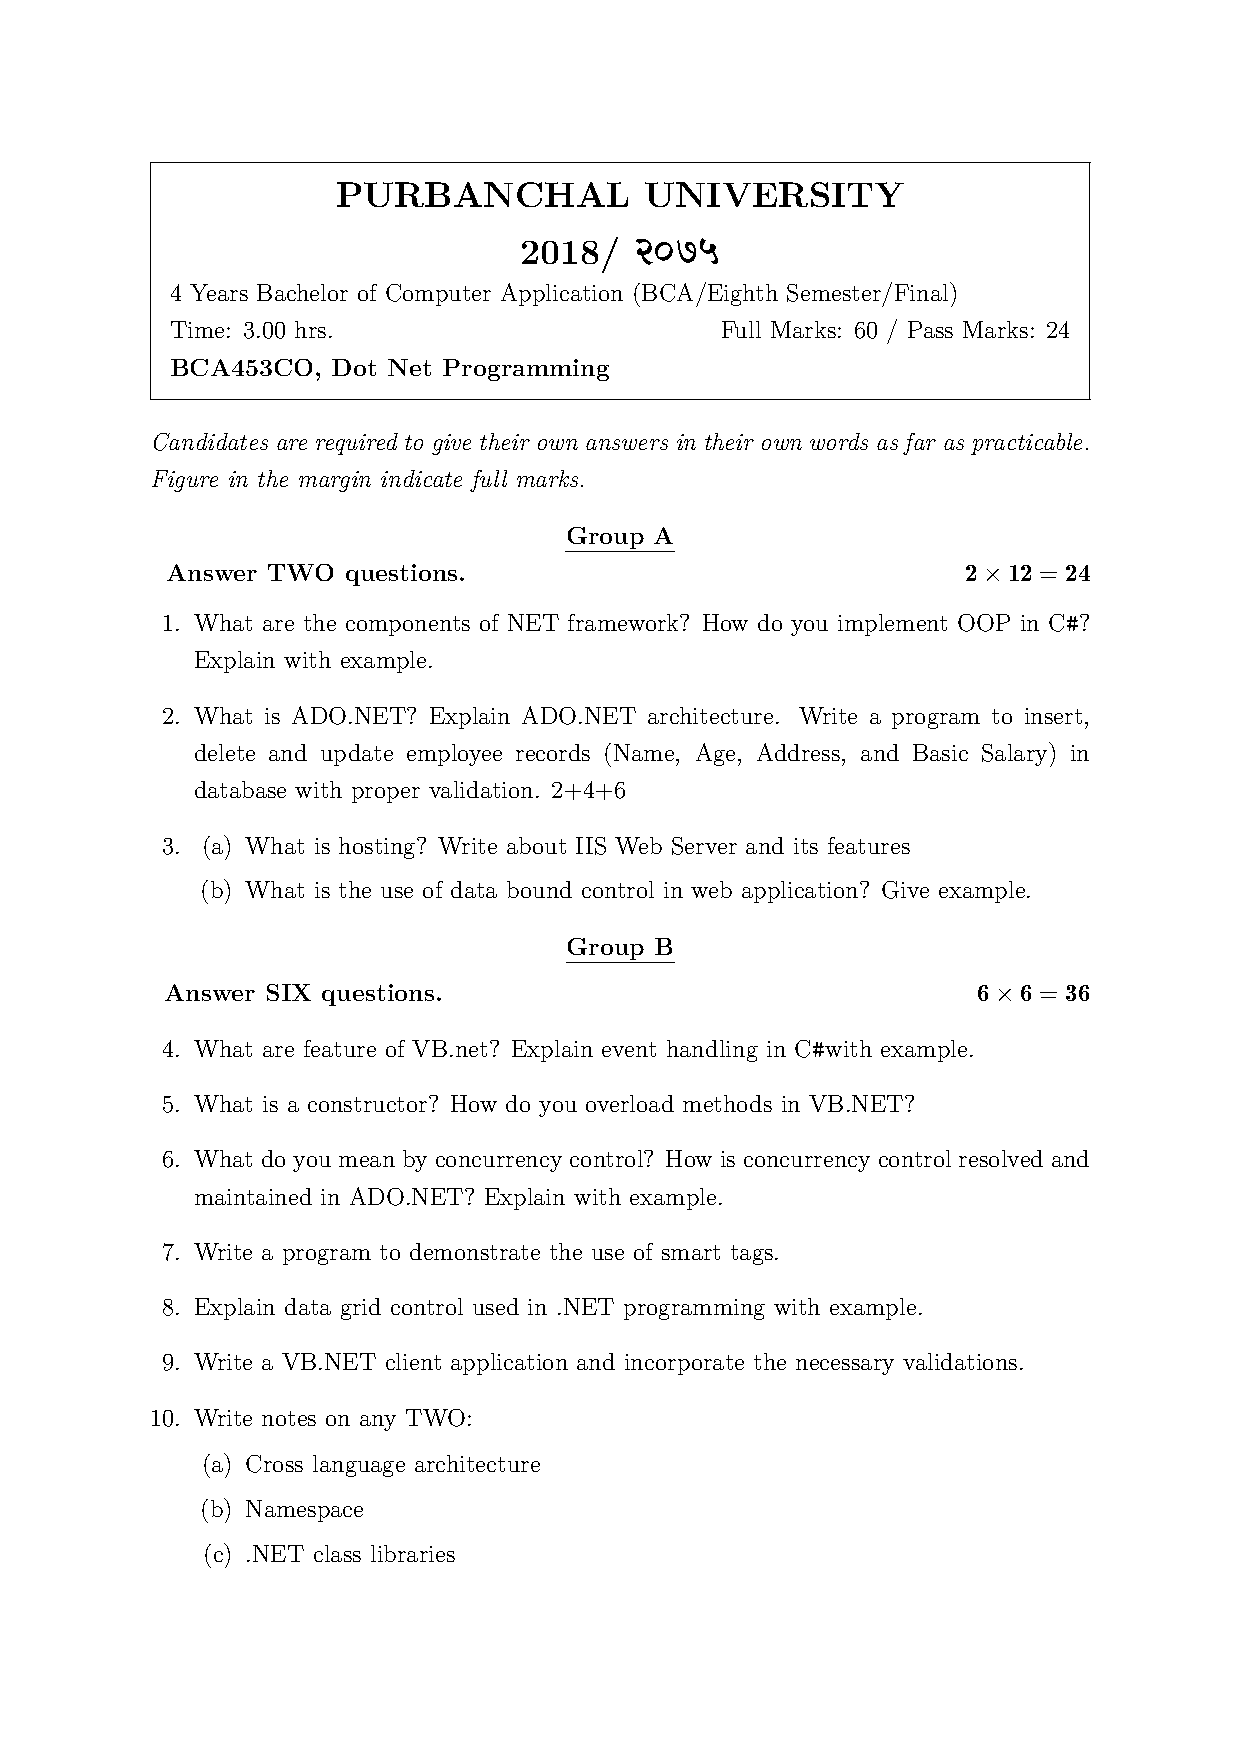
\includepdf[pagecommand={\thispagestyle{plain}}, pages={1-4}, scale=1.00]{./questions/dot_net_programming_questions}




\backmatter

%-----------------------------------------
%		References
%-----------------------------------------
 \nocite{*}
 \renewcommand{\bibname}{References}
 \phantomsection
 \addcontentsline{toc}{chapter}{References}
 \printbibliography 
 

\end{document}
